\documentclass[12pt, a4paper]{article}

\usepackage{float}
\restylefloat{table}
\usepackage{parskip}
\usepackage{graphicx}
\usepackage{caption}
\usepackage{ragged2e}
\graphicspath{{./images/}}

\title{Proiect Baze de Date}
\author{George Radu}
\date{}

\begin{document}
\maketitle

\section{Introducere}
\quad \par
Detaliile din acest proiect se referă la proiectarea unui model de date ce furnizează informații despre gestiunea companiilor de transporturi rutiere de mărfuri din România.

Modelul de date va gestiona informații legate de transporturile de mărfuri ale unor companii client de un depozit la altul. Există firme de pază care se ocupă de paza depozitelor. O firmă de pază alocă fiecărui depozit o echipă de pază.

Transporturile de marfă sunt realizate de o firmă de transport prin intermediul angajaților profesioniști care pot avea mai multe categorii de permise și se pot opri la mai multe popasuri petru odihnă/masă/alimentare. Transportul de marfă începe de la un depozit și se termină la alt depozit, în fiecare depozit accesul camionului este permis dupa o verificare a echipei de pază.

\section{Restricții de funcționare}
\quad \par
Modelul de date respectă anumite restricții de funcționare.
\begin{itemize}
    \item Orice depozit are un singur deținător(o companie client ori o firmă de transport) și poate fi folosit pentru depozitarea de mărfuri.
    \item O companie client sau o firmă de transport poate deține mai multe depozite.
    \item Unui depozit îi este alocată o unică locație.
    \item Un depozit este păzit la un moment dat de o singură echipă de pază.
    \item Un depozit are o listă de inventar cu ce mărfuri au intrat/ieșit împreună cu data și ora.
    \item Un lot de marfă poate să fie transportat de mai multe ori, nu neapărat î1 același transport, și nu neapărat între aceleași depozite.
    \item O echipă de pază aparține unei firme de pază, firmă de pază care poate avea mai multe echipe de pază care să păzească mai multe depozite aflate în diferite locații.
    \item Un angajat poate să fie ori paznic ori șofer.
    \item Un transport de marfă se realizează prin intermediul unui camion \\încărcat cu marfă de la un depozit la altul.
    \item Un șofer poate să oprească în timpul transportului la mai multe popasuri pentru odihnă/mâncare sau alimentare. La popasuri pot veni mai mulți șoferi.
    \item Un popas se află intr-o unică locație și poate fi o benzinărie, un motel sau un restaurant. Nu ne interesează detalii specifice despre un popas cum ar fi ce mâncare vinde un restaurant, sau cât costa o cameră la un motel.
    \item Un șofer poate să aibă mai multe permise pentru mai multe categorii, poate chiar să i se anuleze un permis și să trebuiască să îl obțină din nou.
    \item Un șofer trebuie să conducă un camion, dar poate să conducă mai multe camioane(nu in acelasi timp) în funcție de problemele tehnice legate de camion și necesitățile firmei.
    \item O firmă de transport deține mai multe camioane, iar un camion este deținut de o singură firmă de transport.
    \item Transportul de marfă se face între 2 depozit, se transportă mai multe loturi de marfă. Pentru un transport vom reține și data din momentul în care a început transportul. Pentru fiecare transport se va folosi un singur camion condus de un șofer profesionist.
\end{itemize}

\section{Entități}
\quad \par
Pentru modelul de date referitor la gestiunea companiilor de transporturi rutiere de mărfuri, structurile: DEPOZIT, LOCATIE, POPAS, FIRMA, CLIENT, PAZA, TRANSPORT, ECHIPA\_PAZA, INVENTAR\_DEPOZIT, INVENTAR\_TRANSPORT, LOT\_MARFA, CAMION, ANGAJAT,\\ PAZNIC, SOFER, PERMIS reprezintă entități.

Vom prezenta entitățile modelului de date, realizând o descriere completă a fiecăreia. De asemnea, pentru fiecare entitate se va preciza cheia primară.

Toate entitățile care vor fi precizate sunt independente, cu excepția\\ entităților dependente ECHIPA\_PAZA, PERMIS și\\ INVENTAR\_TRANSPORT
și a subentităților SOFER, PAZNIC, CLIENT, PAZA, TRANSPORT.

\begin{itemize}
    \item DEPOZIT = entitatea descrie o construcție al cărei proprietar este o firmă client sau de transport, în care pot fi depozitate mărfuri. Cheia primară a entității este id\_depozit.
    \item LOCATIE = entitatea descrie informații despre locația fizică a unei construcții, fie ea depozit sau popas. Cheia primară a entității este id\_locatie.
    \item POPAS = reprezintă un loc în care un șofer se poate opri pentru odihnă. Cheia primară a entității este id\_popas.
    \item FIRMA = entitatea descrie o persoană juridică din România, supraentitate pentru CLIENT, PAZA și TRANSPORT. Cheia primară a entității este id\_firma.
    \item CLIENT = persoană juridică beneficiară a unor servicii de transport oferite de o firmă de transport specializată. Cheia primară a entității este id\_firma.
    \item PAZA = persoana juridică ce asigură securitatea depozitelor prin intermediul unor echipe de pază formate din paznici profesioniști. Cheia primară a entității este id\_firma\_paza.
    \item TRANSPORT = persoană juridică responsabilă de transportul de\\ mărfuri în siguranță pentru companii client de la un depozit la altul. Pentru transporturi firma pune la dispoziție șoferilor săi mai multe camioane. Cheia primară a entității este id\_firma\_transport.
    \item ECHIPA\_PAZA = entitatea descrie informații despre o echipă formată din paznici responsabili de securitatea unui depozit. Cheia primară a entității este id\_echipa\_paza.
    \item INVENTAR\_DEPOZIT = entitatea descrie informații despre inventarierea unui depozit, ce loturi au intrat în inventariere, când au intrat și când au ieșit. Cheia primară a entității este id\_inventar\_depozit.
    \item INVENTAR\_TRANSPORT = entitatea descrie informații despre ce lot de marfă a fost implicat intr-un transport între 2 depozite. Cheia primară a entității este cheia compusa dintre id\_inventar\_transport și id\_lot\_marfa.
    \item LOT\_MARFA = entitatea descrie informații despre un lot de marfă transportată sau depozitată. Cheia primară a entității este id\_marfa.
    \item CAMION = vehicul de mare tonaj pentru transport marfă. Cheia primară a entității este id\_camion.
    \item ANGAJAT = persoană fizică angajată a unei companii fie de pază fie de transport pentru a-și oferi serviciile în schimbul unei remunerații. Cheia primară a entității este id\_angajat.
    \item PAZNIC = subentitate a entității ANGAJAT, lucrează pentru o companie de pază și este responsabil de securitatea unui depozit din cadrul echipei sale. Cheia primară a entității este id\_angajat.
    \item SOFER = subentitate a entității ANGAJAT, lucrează pentru o firmă de transport, îi este alocat un camion și este responsabil pentru transportul in siguranță a unei remorci cu marfă. Cheia primară a entității este id\_angajat.
    \item PERMIS = entitate ce descrie informații despre ce tipuri de permis are un șofer și când le-a obținut. Cheia primară a entității este una compusă din id\_permis + id\_angajat.
\end{itemize}

\section{Relații}
\quad\newline
Se vor prezenta relațiile modelului de date, dând o descriere completă a fiecăreia. Denumirile acestor legături între entități sunt alese sugestiv. Pentru fiecare relație se va preciza cardinalitatea minimă și maximă.
\begin{itemize}
    \item DEPOZIT\_se\_află\_LOCATIE = relație ce leagă entitățile DEPOZIT și LOCATIE, reflectând legătura dintre acestea(un depozit se află plasat într-o locație unică din țară). Ținând cont de condițiile impuse modelului un depozit trebuie să se afle într-o singură locație. Relația are cardinalitatea minimă 1:1 și cardinalitatea maximă 1:1.
    \item POPAS\_se\_află\_LOCATIE = relație ce leagă entitățile POPAS și  LOCATIE, reflectând legătura dintre acestea(un popas se află plasat într-o locație unică din țară). Ținând cont de condițiile impuse modelului un popas trebuie să se afle într-o singură locație. Relația are cardinalitatea minimă 1:1 și cardinalitatea maximă 1:1.
    \item FIRMA\_detine\_DEPOZIT = relație ce leagă entitățile FIRMA și DEPOZIT, reflectând legătura dintre acestea(un depozit este deținut de o firmă). Relația are cardinalitatea minimă 1:1 si cardinalitatea maximă 1:M.
    \item PAZA\_aparține\_ECHIPA\_PAZA = relație ce leagă entitățile PAZA și ECHIPA\_PAZA, reflectând legătura dintre acestea(o echipă de pază aparține unei firme de pază). Relația are cardinalitatea minimă 1:1 si cardinalitatea maximă 1:M.
    \item ECHIPA\_PAZA\_păzește\_DEPOZIT = relație ce leagă entitățile \\ECHIPA\_PAZA și DEPOZIT, reflectând legătura dintre acestea (o echipă de pază trebuie să păzească un depozit pentru a permite accesuri în depozit doar de staff autorizat). Relația are cardinalitatea minimă 1:1 si cardinalitatea maximă 1:1(Conform condițiilor impuse modelului un depozit va fi păzit la un moment în timp doar de o echipă de pază).
    \item PAZNIC\_aparține\_ECHIPA\_PAZA = relație ce leagă entitățile PAZNIC și ECHIPA\_PAZA, reflectând legătura dintre acestea (un paznic trebuie să facă parte dintr-o echipă de pază trimisă la un depozit, paznicul lucrează pentru firmă de pază de care aparține echipa). Relația are cardinalitatea minimă 1:1 si cardinalitatea maximă M:1(un paznic face parte dintr-o singură echipă, iar o echipă este formată din mai mulți paznici).
    \item INVENTAR\_DEPOZIT\_aparține\_DEPOZIT = relație ce leagă entită-țile INVENTAR\_DEPOZIT și DEPOZIT, reflectând legătura dintre acestea (un depozit trebuie să țină inventarul la ce loturi de marfă intră și iese și când s-au întâmplat aceste evenimente). Relația are cardinalitatea minimă 0:1 si cardinalitatea maximă M:1(inițial un depozit abia construit poate să nu conțină niciun record de invetariere, urmând pe parcurs să aibă).
    \item INVENTAR\_DEPOZIT\_aparține\_LOT\_MARFA = relație ce leagă entitățile INVENTAR\_DEPOZIT și LOT\_MARFA , reflectând legătura dintre acestea(un lot de marfă va fi înregistrat în lista de inventar a unui depozit atunci când va fi adus în depozit fizic). Relația are cardinalitatea minimă 1:1 si cardinalitatea maximă M:1(Același lot de marfă poate să fie transferat între depozite din puncte cheie din țarâ în funcție de necesitățile firmei client).
    \item LOT\_MARFA\_aparține\_INVENTAR\_TRANSPORT = relație ce leagă entitățile LOT\_MARFA și INVENTAR\_TRANSPORT, reflectând \\legătura dintre acestea (pentru fiecare transport de marfă se face un inventar din care fac parte mai multe loturi de marfă, un lot de marfă poate să fie transportat de mai multe ori). Relația are cardinalitatea minimă 1:1 si cardinalitatea maximă 1:M(ținând cont de condițiile impuse modelului entitatea INVENTAR\_TRANSPORT va conține doar un lot de marfă și din ce lot face parte).
    \item CAMION\_transportă\_INVENTAR\_MARFĂ\_de\_la\_DEPOZIT\\\_la\_DEPOZIT = relație de tip 3 leagă entitățile DEPOZIT, DEPOZIT, INVENTAR\_MARFĂ și CAMION, reflectând ce marfă a fost transportată de la un depozit de plecare la unul de sosire, transportul fiind făcut cu un camion. Denumirea acestei relații va fi transport.
    \item TRANSPORT\_detine\_CAMION = relație ce leagă entitățile TRANSPORT și CAMION, reflectând legătura dintre acestea(o firmă de transport trebuie să dețină camioane). Relația are cardinalitatea minimă 1:1 si cardinalitatea maximă 1:M.
    \item SOFER\_conduce\_CAMION = relație ce leagă entitățile SOFER și \\CAMION, reflectând legătura dintre acestea(un șofer de la o firmă de transport trebuie să conducă cel puțin un camion pentru a-și îndeplini saricinile de la muncă). Relația are cardinalitatea minimă 1:1 si cardinalitatea maximă M:M.
    \item ANGAJAT\_lucrează\_la\_FIRMA = relație ce leagă entitățile ANGAJAT și FIRMA, reflectând legătura dintre acestea(un anagajt/o persoană fizică este angajat/ă la o firmă, acesta își oferă serviciile în schimbul unei remunerații). Relația are cardinalitatea minimă 1:1 si cardinalitatea maximă M:1.
    \item SOFER\_detine\_PERMIS = relație ce leagă entitățile SOFER și PERMIS, reflectând legătura dintre acestea(un șofer pentru a se putea angaja are nevoie de un permis care să îi ofere dreptul de a conduce un camion, șoferul poate să aibă mai multe categorii de permise, în functie de necesitățile sale). Relația are cardinalitatea minimă 1:1 si cardinalitatea maximă 1:M.
    \item SOFER\_istoric\_popasuri\_POPAS = relație ce leagă entitățile SOFER și POPAS, reflectând legătura dintre acestea(un șofer nu poate să conducă mai mult de 8h conform legii, motiv pentru care trebuie să mai ia pauze de odihnă, pauze pe care le poate lua la un motel sau în parcarea unui restaurant sau benzinării de unde poate să și mănânce și să se întâlnească cu alți șoferi). Relația are cardinalitatea minimă 0:0 si cardinalitatea maximă M:M.

\end{itemize}

\section{Atribute}
\begin{itemize}
    \item Entitatea independentă LOCATIE are ca atribute:
        \begin{itemize}
            \item id\_locatie = variabilă de tip întreg, de lungime maximă 10, care reprezintă id-ul unei locații.
            \item județ = variabilă de tip caracter, de lungime maximă 25, care reprezintă numele județului.
            \item localitate = variabilă de tip caracter, de lungime maximă 25, care reprezintă numele localității.
            \item stradă = variabilă de tip caracter, de lungime maximă 25, care reprezintă numele străzii.
            \item nr = variabilă de tip întreg, de lungime maximă 5, care reprezintă numărul locației.
        \end{itemize}
    \item Entitatea independentă DEPOZIT are ca atribute:
        \begin{itemize}
            \item id\_depozit = variabilă de tip întreg, de lungime maximă 5, care reprezintă id-ul unui depozit.
            \item id\_locatie = variabilă de tip întreg, de lungime maximă 10, care reprezintă id-ul locației pentru depozit. Atributul trebuie să corespundă la o valoare a cheii primare din tabelul LOCATIE.
            \item id\_firma = variabilă de tip întreg, de lungime maximă 12, care reprezintă id-ul firmei care deține depozitul. Atributul trebuie să corespundă la o valoare a cheii primare din tabelul FIRMA.
            \item id\_echipa\_paza = variabilă de tip întreg, de lungime maximă 5, care reprezintă id-ul echipei de pază al depozitului. Atributul trebuie să corespundă la o valoare a cheii primare din tabelul ECHIPA\_PAZA.
        \end{itemize}
    \item Entitatea independentă POPAS are ca atribute:
        \begin{itemize}
            \item id\_popas = variabilă de tip întreg, de lungime maximă 10, care reprezintă id-ul unui popas.
            \item id\_locatie = variabilă de tip întreg, de lungime maximă 10, care reprezintă id-ul locației pentru popas. Atributul trebuie să corespundă la o valoare a cheii primare din tabelul LOCATIE.
            \item nume = variabilă de tip caracter, de lungime maximă 25, care reprezintă numele popasului.
            \item tip\_popas = variabilă de tip caracter, de lungime maximă 10. Atributul poate lua valorile: BENZINĂRIE, MOTEL, RESTAURANT.
        \end{itemize}
    \item Entitatea independentă FIRMA are ca atribute:
        \begin{itemize}
            \item id\_firma = variabilă de tip întreg, de lungime maximă 12, care reprezintă id-ul firmei.
            \item nume = variabilă de tip caracter, de lungime maximă 25, care reprezintă numele firmei, numele unei firme este unic.
            \item tip\_firmă = variabilă de tip caracter, de lungime maximă 10, care poate lua valorile: CLIENT, PAZA, TRANSPORT.
        \end{itemize}
    \item Entitatea ECHIPA\_PAZA are ca atribute:
        \begin{itemize}
            \item id\_echipa\_paza = variabilă de tip întreg, de lungime maximă 5, care reprezintă id-ul unei echipe din cadrul firmei de pază.
            \item id\_firma = variabilă de tip întreg, de lungime maximă 12, care reprezintă id-ul firmei de pază. Atributul trebuie să corespundă la o valoare a cheii primare din tabelul PAZA.
        \end{itemize}
    \item Entitatea INVENTAR\_DEPOZIT are ca atribute:
        \begin{itemize}
            \item id\_inventar\_depozit = variabilă de tip întreg de lungime maximă 10, care reprezintă id-ul unei intrări de marfă în inventar.
            \item id\_depozit = variabilă de tip întreg, de lungime maximă 5, care reprezintă id-ul depozitul în care se află marfa. Atributul trebuie să corespundă la o valoare a cheii primare din tabelul .
            \item id\_lot\_marfa = variabilă de tip întreg, de lungime maximă 10, care reprezintă id-ul lotului de marfă care a intrat în inventar. Atributul trebuie să corespundă la o valoare a cheii primare din tabelul LOT\_MARFA.
            \item data\_sosire = variabilă de tip data calendaristică, care reprezintă data la care a intrat marfa în inventariere.
            \item ora\_sosire = variabilă de tip ora, care reprezintă ora la care a intrat marfa în inventariere.
            \item data\_plecare = variabilă de tip data calendaristică, care reprezintă data la care a ieșit marfa din inventariere.
            \item ora\_plecare = variabilă de tip ora, care reprezintă ora la care a ieșit marfa din inventariere.
        \end{itemize}
    \item Entitatea LOT\_MARFA are ca atribute:
        \begin{itemize}
            \item id\_lot\_marfa = variabilă de tip întreg, de lungime maximă 10, care reprezintă id-ul unui lot de marfă.
            \item nume = variabilă de tip caracter, de lungime maximă 25, care reprezintă numele mărfii din lot.
            \item cantitate = variabilă de tip real, de lungime maximă 10, care reprezintă cantitatea lotului de marfă.
        \end{itemize}
    \item Entitatea INVENTAR\_TRANSPORT are ca atribute:
        \begin{itemize}
            \item id\_inventar\_transport = variabilă de tip întreg, de lungime maximă 10, care reprezintă id-ul unei intrări de inventar al unui transport.
            \item id\_lot\_marfa = variabilă de tip întreg, de lungime maximă 10, care reprezintă id-ul unui lot de marfă care face parte din inventarul unui transport. Atributul trebuie să corespundă la o valoare a cheii primare din tabelul LOT\_MARFA.
            \item id\_transport = variabilă de tip întreg, de lungime maximă 10, care reprezintă id-ul transportului din care face parte această listare. Atributul trebuie să corespundă la o valoare a cheii primare din tabelul TRANSPORT.
        \end{itemize}
    \item Entitatea TRANSPORT are ca atribute:
        \begin{itemize}
            \item id\_transport = variabilă de tip întreg, de lungime maximă 10, care reprezintă id-ul unui transport de marfă între 2 depozite.
            \item depozit\_plecare = variabilă de tip întreg, de lungime maximă 5, care reprezintă id-ul depozitului de unde începe transportul și este preluată marfa. Atributul trebuie să corespundă la o valoare a cheii primare din tabelul DEPOZIT.
            \item depozit\_destinație = variabilă de tip întreg, de lungime maximă 5, care reprezintă id-ul depozit unde este livrată marfa. Atributul trebuie să corespundă la o valoare a cheii primare din tabelul DEPOZIT.
            \item id\_camion = variabilă de tip întreg, de lungime maximă 5, care reprezintă id-ul camionului folosit pentru transport. Atributul trebuie să corespundă la o valoare a cheii primare din tabelul CAMION.
            \item data\_plecare = variabilă de tip data calendaristică, care reprezintă data la care a plecat camionul din depozitul de plecare.
            \item ora\_plecare = variabilă de tip ora, care reprezintă ora la care a plecat camionul din depozitul de plecare.
        \end{itemize}
    \item Entitatea CAMION are ca atribute:
        \begin{itemize}
            \item id\_camion = variabilă de tip întreg, de lungime maximă 5, care reprezintă id-ul unui camion.
            \item id\_firma = variabilă de tip întreg, de lungime maximă 12, care reprezintă id-ul firmei de transport care deține camionul. Atributul trebuie să corespundă la o valoare a cheii primare din tabelul TRANSPORT.
            \item marca = variabila de tip caracter, de lungime maxima 10, care reprezinta firma care a produs camionul.
            \item nr\_inmatriculare = variabila de tip caracter, de lungime maxima 10, reprezinta un identificator unic pentru autovehicule. Acest atribut poate fi schimbat (de obicei cand se se schimba detinatorul) motiv pentru care nu reprezinta parte din cheia primara.
        \end{itemize}
    \item Entitatea ANGAJAT are ca atribute:
        \begin{itemize}
            \item id\_angajat = variabilă de tip întreg, de lungime maximă 10, care reprezintă id-ul unui angajat.
            \item nume = variabilă de tip caracter, de lungime maximă 25, care reprezintă numele unui angajat.
            \item prenume = variabilă de tip caracter, de lungime maximă 25, care reprezintă prenumele unui angajat.
            \item nr\_telefon = variabilă de tip caracter, de lungime maximă 14, care reprezintă numărul de telefon al unui angajat.
            \item data\_angajare = variabilă de tip data calendaristică, care \\reprezintă data în care a fost angajat o persoană.
            \item salariu = variabilă de tip real, de lungime maximă 10, care repre-zintă salariul anagajatului.
            \item id\_firma = variabile de tip întreg, de lungime maximă 12, care reprezintă id-ul firmei la care lucrează angajatul. Atributul trebuie să corespundă la o valoare a cheii primare din tabelul FIRMA.
            \item tip\_angajat = variabilă de tip caracter, de lungime maximă 6, care reprezintă tipul angajatului. Poate să fie PAZNIC sau SOFER.
        \end{itemize}
    \item Entitatea PAZNIC are aceleași atribute ca supraentitatea din care face parte + atributul id\_echipa\_paza (= variabilă de tip întreg, de lungime maximă 5, care reprezintă id-ul echipei de pază din care face parte paznicul. Atributul trebuie să corespundă la o valoare a cheii primare din tabelul ECHIPA\_PAZA).
    \item Entitatea SOFER are aceleași atribute ca supraentitatea din care face parte. Nu are alte atribute adiționale.
    \item Entitatea ISTORIC\_CAMIOANE\_CONDUSE are ca atribute:
        \begin{itemize}
            \item id\_istoric\_camioane\_conduse = variabilă de tip întreg, de lungime maximă 10, care reprezintă id-ul unei intrări în istoric.
            \item id\_angajat = variabilă de tip întreg, de lungime maximă 10, care reprezintă id-ul unui șofer. Atributul trebuie să corespundă la o valoare a cheii primare din tabelul SOFER.
            \item id\_camion = variabilă de tip întreg, de lungime maximă 5, care reprezintă id-ul camionului condus. Atributul trebuie să corespundă la o valoare a cheii primare din tabelul CAMION.
            \item data\_inceput = variabilă de tip data calendaristică, care reprezintă data la care a început un șofer să conducă un camion al firmei de transport.
            \item data\_sfarsit = variabilă de tip data calendaristică, care reprezintă data la care un șofer nu mai conduce un camion.
        \end{itemize}
    \item Entitatea PERMIS are ca atribute:
        \begin{itemize}
            \item id\_permis = variabilă de tip întreg, de lungime maximă 10, care reprezintă id-ul unui permis.
            \item id\_angajat = variabilă de tip întreg, de lungime maximă 10, care reprezintă id-ul unui angajat care deține un permis. Atributul trebuie să corespundă la o valoare a cheii primare din tabelul SOFER.
            \item categorie = variabilă de tip caracter, de lungime maximă 3, care reprezintă tipul de permis care poate fi deținut de o persoană. Atributul poate lua valorile AM, A1, A2, A, B1, B, BE, C1, C1E, C, CE, D1, D1E, D, DE, Tr, Tb sau Tv.
            \item data = variabilă de tip data calendaristică, care reprezintă data la care a fost emis permisul pentru o persoană.
            \item ora = variabilă de tip ora, care reprezintă ora la care a fost emis permisul pentru o persoană.
        \end{itemize}
    \item Entitatea ISTORIC\_POPASURI are ca atribute:
        \begin{itemize}
            \item id\_istoric\_popas = variabilă de tip întreg, de lungime maximă 20, care reprezintă id-ul unui istoric în popas.
            \item id\_popas = variabilă de tip întreg, de lungime maximă 10, care reprezintă id-ul unui popas la care s-a oprit un șofer. Atributul trebuie să corespundă la o valoare a cheii primare din tabelul POPAS.
            \item id\_angajat = variabilă de tip întreg, de lungime maximă 10, care reprezintă id-ul unui șofer care s-a oprit la un popas. Atributul trebuie să corespundă la o valoare a cheii primare din tabelul SOFER.
            \item data\_sosire = variabilă de tip data calendaristică, care reprezintă data la care a ajuns un șofer la un popas.
            \item ora\_sosire = variabilă de tip ora, care reprezintă ora la care a ajuns un șofer la un popas.
            \item data\_plecare = variabilă de tip data calendaristică, care reprezintă data la care a plecat un șofer de la un popas.
            \item ora\_plecare = variabilă de tip ora, care reprezintă ora la care a plecat un șofer de la un popas.
        \end{itemize}
\end{itemize}

    Mai sunt de prezentat următoarele relații care se vor transforma in tabele asociative:
\begin{itemize}
    \item Relația CAMION\_transportă\_INVENTAR\_MARFĂ\_de\_la\_DEPOZIT\\\_la\_DEPOZIT are ca atribute: id\_transport, depozit\_plecare,\\ depozit\_destinație, camion, data\_plecare, ora\_plecare.
    \item Relația SOFER\_conduce\_CAMION are ca atribute: \\id\_istoric\_camioane\_conduse, id\_angajat, id\_camion, data\_inceput,\\ data\_sfarsit.
    \item Relația SOFER\_istoric\_popasuri\_POPAS are ca atribute: \\id\_istoric\_popas, id\_popas, id\_angajat, data\_sosire, ora\_sosire,\\ data\_plecare, ora\_plecare.
\end{itemize}

\newpage
\section{Diagrama entitate-relație E/R}
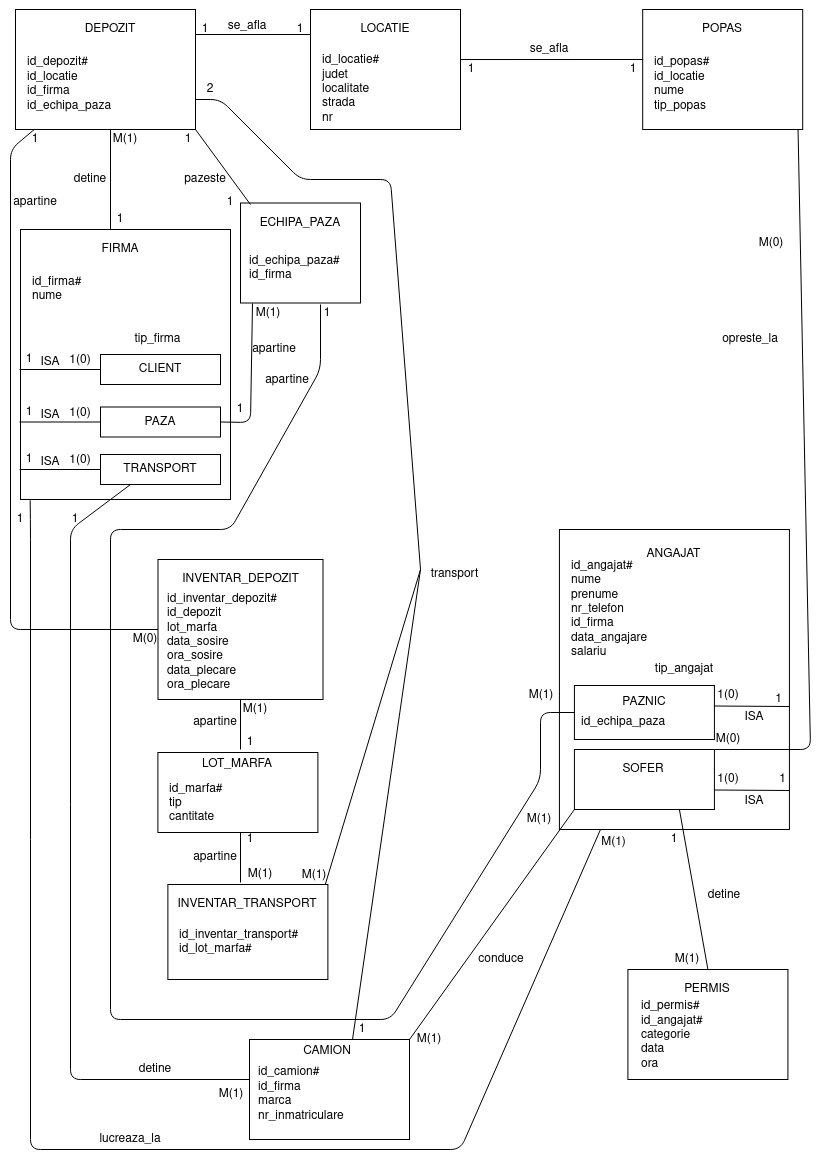
\includegraphics[width=\textwidth]{_diagrama_er.png}
\label{Figura 1}
\centering Figura 1

\justify

\section{Diagrama conceptuală}
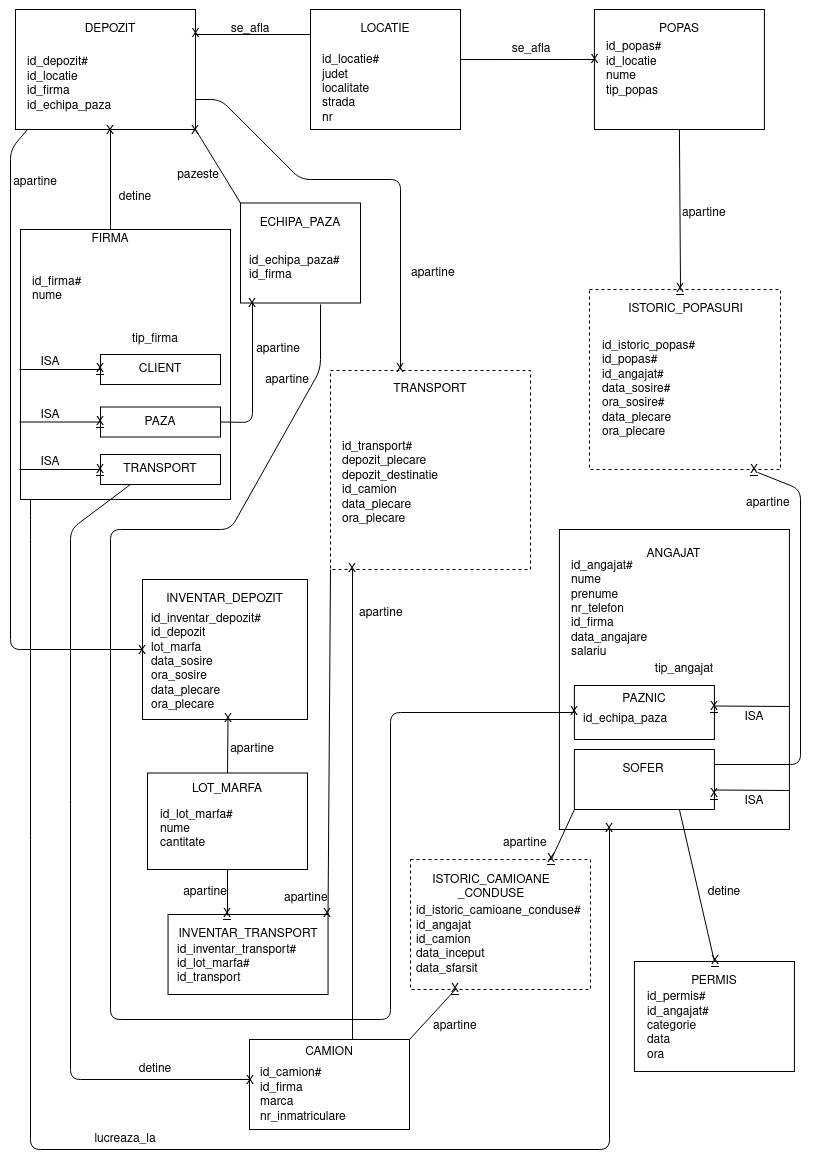
\includegraphics[width=\textwidth]{_diagrama_conceptuala.png}
\label{Figura 2}
\centering Figura 2

\justify

\section{Schemele relaționale}
\quad \par
Schemele relaționale corespunzătoare diagramei conceptuale din Figura 2 sunt următoarele:
\begin{itemize}
    \item DEPOZIT(id\_depozit\#, id\_locatie, id\_echipa\_paza, id\_firma)
    \item LOCATIE(id\_locatie\#, județ, localitate, stradă, nr)
    \item POPAS(id\_popas\#, id\_locatie, nume, tip\_popas)
    \item FIRMA(id\_firma\#, nume, tip\_firmă)
    \item CLIENT(id\_firma\#)
    \item PAZA(id\_firma\#)
    \item TRANSPORT(id\_firma\#)
    \item ECHIPA\_PAZA(id\_echipa\_paza\#, id\_firma\_paza)
    \item INVENTAR\_DEPOZIT(id\_inventar\_depozit\#, id\_depozit, \\id\_lot\_marfa, data\_sosire, ora\_sosire, data\_plecare, ora\_plecare)
    \item INVENTAR\_TRANSPORT(id\_inventar\_transport\#, id\_marfa\#,\\ id\_transport)
    \item LOT\_MARFA(id\_lot\_marfa\#, nume, cantitate)
    \item CAMION(id\_camion\#, id\_firma, marca, nr\_inmatriculare)
    \item TRANSPORT(id\_transport\#, depozit\_plecare, depozit\_destinație,\\ id\_camion, data\_plecare, ora\_plecare)
    \item ANGAJAT(id\_angajat\#, nume, prenume, nr\_telefon, data\_angajare, salariu, id\_firma, tip\_angajat)
    \item PAZNIC(id\_angajat\#, id\_echipa\_paza)
    \item SOFER(id\_angajat\#)
    \item PERMIS(id\_permis\#, id\_angajat\#, categorie, data, ora)
    \item ISTORIC\_CAMIOANE\_CONDUSE(id\_istoric\_camioane\_conduse\#,\\ id\_angajat, id\_camion, data\_inceput, data\_sfarsit)
    \item ISTORIC\_POPASURI(id\_istoric\_popas\#, id\_popas\#, id\_angajat\#,\\ data\_sosire, ora\_sosire, data\_plecare, ora\_plecare)
\end{itemize}

\section{Forme normale}

\subsection*{Exemplu 1}
Se dă relația \emph{SOFER\_detine\_PERMIS} în care un șofer poate deține mai multe permise. S-a plecat de relația de tipul(obs. nu sunt trecute toate atributele unui angajat, doar câteva pentru a nu mări tabelul și a face toate datele cât mai lizibile și clare):

\begin{table}[!htbp]
\caption{Relația nu e în FN1}\label{tab1}
\resizebox{\columnwidth}{!}{\begin{tabular}{| l | l | l | l | l | l | l | l | l | l | l |}
\hline
id\_angajat\# & nume & prenume & .. & tip\_angajat & id\_permis\# & categorie & data & ora \\
\hline
20000 & Ion & Vasile  & .. & SOFER & 1 & C, B, A & 06-06-2012, & 12$:$00, \\
 & & & & & & & 06-06-2013, & 12$:$00, \\
 & & & & & & & 06-06-2017 & 12$:$00 \\
\hline
20020 & Ovidie & Ion & .. & SOFER & 2 & C & 06-06-2018 & 12$:$00 \\
\hline
20100 & Constantin & Gheorghe & .. & SOFER & 3 & B, C & 06-06-2010, & 12$:$00, \\
 & & & & & & & 06-06-2012 & 12$:$00 \\
\hline
\end{tabular}}
\end{table}

în care se observă că atributelor \emph{categorie}, \emph{data} și \emph{ora} le corespund o listă de valori, i.e. nu le corespund o valoare indivizibilă(atomică), de unde se trage concluzia că relația \emph{SOFER\_detine\_PERMIS} nu se află în forma normala 1 (FN1). Se aduce relația în FN1 spărgând atributele nonatomice în atribute atomice, proces în care se adaugă mai multe linii pentru fiecare categorie de permis pentru un șofer după cum urmează:

\begin{table}[!htbp]
\caption{Transformarea în FN1}\label{tab2}
\resizebox{\columnwidth}{!}{\begin{tabular}{| l | l | l | l | l | l | l | l | l | l | l |}
\hline
id\_angajat\# & nume & prenume & .. & tip\_angajat & id\_permis\# & categorie & data & ora \\
\hline
20000 & Ion & Vasile  & .. & SOFER & 1 & A & 06-06-2012 & 12$:$00 \\
\hline
20000 & Ion & Vasile  & .. & SOFER & 2 & B & 06-06-2013 & 12$:$00 \\
\hline
20000 & Ion & Vasile  & .. & SOFER & 3 & C & 06-06-2017 & 12$:$00 \\
\hline
20020 & Ovidie & Ion & .. & SOFER & 1 & C & 06-06-2018 & 12$:$00 \\
\hline
20100 & Constantin & Gheorghe & .. & SOFER & 1 & B & 06-06-2010 & 12$:$00 \\
\hline
20100 & Constantin & Gheorghe & .. & SOFER & 2 & C & 06-06-2012 & 12$:$00 \\
\hline
\end{tabular}}
\end{table}

Pentru ca relația \emph{SOFER\_detine\_PERMIS} să fie în formă normală 2 (FN2) trebuie să fie mai întâi în FN1, lucru realizat anterior, și în plus trebuie să indeplinească condiția ca fiecare atribut care nu este cheie (nu participă la cheia primară) este \textbf{dependent de întreaga cheie primară}.

Relația de mai sus nu se află în FN2 întrucât se găsesc atributele \emph{nume, prenume, nr\_telefon, .., tip\_angajat} care nu sunt chei și trebuie să depindă direct de întreaga cheie primară \textbf{id\_angajat\#} și \textbf{id\_permis\#}. Atributele nu depind direct de întreaga cheie primară, deoarece se observă dependeța directă dintre \emph{id\_angajat\#} și \emph{nume, prenume, .., tip\_angajat}, însemnând că \emph{nume, prenume, .., tip\_angajat} depind direct doar de o parte a cheii primare(i.e. \emph{id\_angajat\#} nu și de \emph{id\_permis\#}).

Aplicăm regula \emph{Casey-Delobel} pentru FN2:

Avem relația \emph{R(K1, K2, X, Y)}, unde \emph{K1=id\_angajat\#}, \emph{K2=id\_permis\#} care definesc cheia primară compusă, iar \emph{X} și \emph{Y} sunt mulțimi de atribute, astfel încât \emph{K1}$\rightarrow$\emph{X}, unde \emph{X}=\{\emph{nume, prenume, nr\_telefon, .., tip\_angajat}\} și \emph{Y}=\{\emph{categorie, data, ora}\}.

Din cauza dependenței funcționale \emph{K1}$\rightarrow$\emph{X} care arată că \emph{R} nu este în FN2, se înlocuiește R(\emph{fără pierdere de informație}) prin două proiecții: \emph(K1, K2, Y) și \emph(K1, X).

Astfel avem în final proiecțiile:

\begin{itemize}
    \item \{id\_angajat\#\} $\rightarrow$ \{nume, prenume, nr\_telefon, data\_angajare, id\_firma, nume\_firma, tip\_angajat\}, \emph{id\_angajat\#} determinând funcțional\\ atributele menționate anterior
    \item \{id\_permis\#, id\_angajat\#\} $\rightarrow$ \{categorie, data, ora\}
\end{itemize}

\begin{table}[!htbp]
\begin{center}
\caption{Proiectia \emph{R1(K1, K2, Y)}}\label{tab3}
\resizebox{\width}{!}{\begin{tabular}{| l | l | l | l | l | l | l | l | l | l | l |}
\hline
id\_angajat\# & id\_permis\# & categorie & data & ora \\
\hline
20000 & 1 & A & 06-06-2012 & 12$:$00 \\
\hline
20000 & 2 & B & 06-06-2013 & 12$:$00 \\
\hline
20000 & 3 & C & 06-06-2017 & 12$:$00 \\
\hline
20020 & 1 & C & 06-06-2018 & 12$:$00 \\
\hline
20100 & 2 & B & 06-06-2010 & 12$:$00 \\
\hline
20100 & 1 & C & 06-06-2012 & 12$:$00 \\
\hline
\end{tabular}}
\end{center}
\end{table}

\begin{table}[!htbp]
\begin{center}
\caption{Proiectia \emph{R2(K1, X)}}\label{tab4}
\resizebox{\width}{!}{\begin{tabular}{| l | l | l | l | l |}
\hline
id\_angajat\# & nume & prenume & .. & tip\_angajat \\
\hline
20000 & Ion & Vasile  & .. & SOFER \\
\hline
20020 & Ovidie & Ion & .. & SOFER \\
\hline
20100 & Constantin & Gheorghe & .. & SOFER \\
\hline
\end{tabular}}
\end{center}
\end{table}

Pentru ca relația \emph{SOFER\_detine\_PERMIS} să fie în formă normală 3 (FN3) trebuie să fie mai întâi în FN2, lucru realizat anterior, și în plus trebuie să îndeplinească condiția ca fiecare atribut care nu este cheie(nu participă la o cheie) \textbf{să depindă direct de cheia primară}.

În proiecția \emph{R1(K1, K2, Y)} toate atributele depind direct de cheia primară. \emph{Categoria} reprezintă tipul de autovehicul pe care permisul îi oferă dreptului unui șofer care l-a obținut să conducă autovehicule de categoria respectivă. Data și ora reprezintă când a fost obținut permisul de o persoană(de acum supranumită șofer). Pentru această relație nu există dependențe tranzitive, de unde rezultă ca se află în FN3. Se va denumi această relație \emph{SOFER\_detine\_PERMIS}.

Se verifică acum relația \emph{R2(K1, X)}.

\begin{table}[!htbp]
\begin{center}
\caption{Relația \emph{R2(K1, X)}}\label{tab5}
\resizebox{\columnwidth}{!}{\begin{tabular}{| l | l | l | l | l | l | l | l | l | l | l | l |}
\hline
id\_angajat\# & nume & prenume & nr\_telefon & .. & id\_firma & nume & tip\_firma & tip\_angajat \\
\hline
20000 & Ion & Vasile & 0722123456 & .. & 1100 & Road Logistics & TRANSPORT & SOFER \\
\hline
20020 & Ovidie & Ion & 0727124356 & .. & 1100 & Road Logistics & TRANSPORT & SOFER \\
\hline
20100 & Constantin & Gheorghe & 0735123456 & .. & 1400 & Lextom Trans Asd & TRANSPORT & SOFER \\
\hline
\end{tabular}}
\end{center}
\end{table}

Relația R2 este în FN2 după cum a fost demonstrat anterior, însă nu se află în FN3 întrucât se obvservă că atributele \emph{nume(firmă), tip\_firmă} depind tranzitiv de cheia primară \emph{id\_angajat} prin intermediul atributului \emph{id\_firma}.

Pentru a reduce relația în FN3 se aplică regula \emph{Casey-Delobel}. Relația se descompune, prin eliminarea dependențelor funcționale tranzitive, în \\proiecții.

Avem relația \emph{R(K, $X_1$, $X_2$, $X_3$)}, unde $X_2$=\{\emph{nume(firma), tip\_firma}\} depinde tranzitiv de \emph{K}=\emph{id\_angajat\#}(i.e. cheia primara a lui \emph{R}). Se presupune că $K\rightarrow X_1\rightarrow X_2$. ($X_1$=id\_firma si $X_3$=\{nume, prenume, nr\_telefon, ..\})

Din cauza dependenței funcționale $X_1\rightarrow X_2$ care arată că $R$ nu este în FN3, se înlocuiește $R$ (\textbf{fără pierdere de informație}) prin două proiecții $R1(K, X_1, X_3)$ și $R2(X_1, X_2)$.

\begin{itemize}
    \item \{id\_angajat\#\} $\rightarrow$ \{nume, prenume, nr\_telefon, data\_angajare, salariu, id\_firma, tip\_angajat\}
    \item \{id\_firma\#\} $\rightarrow$ \{nume, tip\_firma\}
\end{itemize}

\begin{table}[!htbp]
\begin{center}
\caption{Proiectia \emph{R2-1(K, $X_1$, $X_3$)}}\label{tab6}
\resizebox{\columnwidth}{!}{\begin{tabular}{| l | l | l | l | l | l | l | l | l | l | l | l |}
\hline
id\_angajat\# & nume & prenume & nr\_telefon & .. & id\_firma & tip\_angajat \\
\hline
20000 & Ion & Vasile & 0722123456 & .. & 1100 & SOFER \\
\hline
20020 & Ovidie & Ion & 0727124356 & .. & 1100 & SOFER \\
\hline
20100 & Constantin & Gheorghe & 0735123456 & .. & 1400 & SOFER \\
\hline
\end{tabular}}
\end{center}
\end{table}
\quad \par

\begin{table}[!htbp]
\begin{center}
\caption{Proiectia \emph{R2-2($K_1$, $K_2$)}}\label{tab7}
\resizebox{\width}{!}{\begin{tabular}{| l | l | l | l | l | l | l | l | l | l | l | l |}
\hline
id\_firma\# & nume & tip\_firma \\
\hline
1100 & Road Logistics & TRANSPORT \\
\hline
1100 & Road Logistics & TRANSPORT \\
\hline
1400 & Lextom Trans Asd & TRANSPORT \\
\hline
\end{tabular}}
\end{center}
\end{table}
\quad \par

\setlength\parskip{\baselineskip}
\subsection*{Exemplu 2}

Se dă relația \emph{CAMION\_transportă\_INVENTAR\_MARFĂ\_de\_la\_\\DEPOZIT\_la\_DEPOZIT} în care prin intermediul unui camion este transportată marfă, marfă pentru care se face o inventariere a transportului de la un depozit la altul. Se pleacă de la prima variantă a relației:

\begin{table}[!htbp]
\begin{center}
\caption{Relația nu e în FN1}\label{tab8-1}
\resizebox{\columnwidth}{!}{\begin{tabular}{| l | l | l | l | l | l | l | l | l | l | l | l |}
\hline
id\_         & depozit\_ &  id\_    & id\_  & id\_echipa & depozit\_    & id\_    & id\_  & id\_echipa \\
transport\#  & plecare\# &  locatie & firma & \_paza     & destinatie\# & locatie & firma & \_paza     \\
\hline
10000        & 3000      & 100      & 4     & 1100       & 500        & 30      & 2     & 100 \\
\hline
10010        & 3000      & 100      & 4     & 1100       & 500        & 30      & 2     & 100 \\
\hline
10020        & 3500      & 120      & 10    & 1200       & 1000       & 50      & 3     & 200 \\
\hline
\end{tabular}}
\end{center}
\begin{center}
\label{tab8-2}
\resizebox{\columnwidth}{!}{\begin{tabular}{| l | l | l | l | l | l | l | l | l | l | l | l |}
\hline
id\_     & id\_  & marca & nr\_          & id\_inventar  & id\_lot   & nume & cantitate & data\_  & ora\_   \\
camion\# & firma &       & inmatriculare & \_transport\# & \_marfa\# &      &           & plecare & plecare \\
\hline
15     & 1100  & VOLVO & CT12FSD       & 100           & 100     & carne miel & 100 & 6-05-2021 & 08$:$00 \\
     &   &  &        & 155           & 105     & carne porc & 300 & &  \\
\hline
25     & 1100  & VOLVO & CT90MMM       & 210           & 110     & carne pui & 250 & 8-05-2021 & 06$:$00 \\
\hline
35     & 1200  & SCANIA & PH13SCN      & 265           & 120     & rosii & 1000 & 6-05-2021 & 08$:$00 \\
\hline
\end{tabular}}
\end{center}
\end{table}

în care se observă că atributelor \emph{id\_inventar\_transport, id\_lot\_marfa,\\ nume(marfa), cantitate} le corespund o listă de valori, i.e. nu le corespund o valoare indivizibilă(atomică), de unde se trage concluzia că relația \emph{CAMION\_\\transportă\_INVENTAR\_MARFĂ\_de\_la\_DEPOZIT\_la\_DEPOZIT} nu se află în forma normală 1 (FN1). Se aduce relația în FN1 spărgând atributele \\nonatomice în atribute atomice, proces în care se adaugă mai multe linii pentru fiecare lot de marfă transportat și detaliile sale după cum urmează:

\begin{table}[H]
\begin{center}
\caption{Transformarea în FN1}\label{tab9-1}
\resizebox{\columnwidth}{!}{\begin{tabular}{| l | l | l | l | l | l | l | l | l | l | l | l |}
\hline
id\_         & depozit\_ &  id\_        & id\_      & id\_echipa     & depozit\_    & id\_        & id\_      & id\_echipa \\
transport\#  & plecare\# &  locatie(dp) & firma(dp) & \_paza(dp)     & destinatie\# & locatie(dd) & firma(dd) & \_paza(dd)  \\
\hline
10000        & 3000      & 100      & 4     & 1100       & 500        & 30      & 2     & 100 \\
\hline
10000        & 3000      & 100      & 4     & 1100       & 500        & 30      & 2     & 100 \\
\hline
10010        & 3000      & 100      & 4     & 1100       & 500        & 30      & 2     & 100 \\
\hline
10020        & 3500      & 120      & 10    & 1200       & 1000       & 50      & 3     & 200 \\
\hline
\end{tabular}}
\end{center}
\begin{center}
\label{tab9-2}
\resizebox{\columnwidth}{!}{\begin{tabular}{| l | l | l | l | l | l | l | l | l | l | l | l |}
\hline
id\_     & id\_     & marca & nr\_          & id\_inventar  & id\_lot   & nume & cantitate & data\_  & ora\_   \\
camion\# & firma(c) &       & inmatriculare & \_transport\# & \_marfa\# &      &           & plecare & plecare \\
\hline
15     & 1100  & VOLVO & CT12FSD       & 100           & 100     & carne miel & 100 & 6-05-2021 & 08$:$00 \\
\hline
15     & 1100  & VOLVO & CT12FSD       & 155           & 105     & carne porc & 300 & 6-05-2021 & 08$:$00 \\
\hline
25     & 1100  & VOLVO & CT90MMM       & 210           & 110     & carne pui & 250 & 8-05-2021 & 06$:$00 \\
\hline
35     & 1200  & SCANIA & PH13SCN      & 265           & 120     & rosii & 1000 & 6-05-2021 & 08$:$00 \\
\hline
\end{tabular}}
\end{center}
\end{table}

Obs: Pentru atributele care se repetă s-a adăugat în paranteză la final un alias, a.î. să fie clar de care cheie depinde.

Pentru ca relația \emph{CAMION\_transportă\_INVENTAR\_MARFĂ\_de\_la\_\\DEPOZIT\_la\_DEPOZIT} să fie în formă normală 2 (FN2) trebuie să fie mai întâi în FN1, lucru realizat anterior, și în plus trebuie să indeplinească condiția ca fiecare atribut care nu este cheie (nu participă la cheia primară) este \textbf{dependent de întreaga cheie primară}.

Relația de mai sus nu se află în FN2 întrucât se găsesc atributele \\\emph{id\_firma(dp), id\_firma(dd),id\_firma(c), marca, nr\_inmatriculare} care nu sunt chei și trebuie să depindă direct de întreaga cheie primară \textbf{id\_transport\#} + \textbf{depozit\_plecare} + \textbf{depozit\_destinatie} + \textbf{id\_camion} + \textbf{id\_inventar\_\\transport\#} + \textbf{id\_lot\_marfa}.
Atributele nu depind direct de întreaga cheie primară, deoarece se observă dependeța directă dintre \emph{id\_camion} și \\\emph{id\_firma(c), marca, nr\_inmatriculare} care nu sunt dependente și de \\\emph{depozit\_destinatie} (de exemplu).

Se mai găsesc următoarele dependențe funcționale:
\begin{itemize}
    \item dependența directă dintre \emph{depozit\_plecare} și \emph{id\_locatie(dp), \\id\_firma(dp), id\_echipa\_paza(dp)} care nu sunt dependente și de \\\emph{depozit\_destinație}.
    \item dependența directă dintre \emph{depozit\_destinatie} și \emph{id\_locatie(dd), \\id\_firma(dd), id\_echipa\_paza(dd)} care nu sunt dependente și de \\\emph{depozit\_plecare}.
\end{itemize}

Atributele rămase care nu sunt chei \emph{nume, cantitate, data\_plecare, \\ora\_plecare} depind de întreaga cheie primară întrucât se consideră legătura pentru nume de exemplu:
\begin{itemize}
    \item id\_transport $\rightarrow$ ce marfă a fost transportată într-un transport.
    \item depozit\_plecare $\rightarrow$ ce marfă a plecat din depozit.
    \item depozit\_destinatie $\rightarrow$ ce marfă va fi transportată către depozit.
    \item id\_camion $\rightarrow$ ce marfă va conține camionul.
    \item id\_inventar\_transport $\rightarrow$ ce marfă face parte din inventarierea transportului.
\end{itemize}

Analog pentru celelalte atribute.

Aplicăm regula \emph{Casey-Delobel} pentru FN2:

Avem relația \emph{R(K1, K2, K3, K4, K5, K6, X, Y, Z, W)}, unde \\
\emph{K1=id\_transport\#}, \emph{K2=depozit\_plecare\#}, \emph{K3=depozit\_destinatie\#}, \\\emph{K4=id\_camion\#}, \emph{K5=id\_inventar\_transport\#}, \emph{K6=id\_lot\_marfa\#} \\care definesc cheia primară compusă, iar \emph{X}, \emph{Y}, \emph{Z} și \emph{W} sunt mulțimi de atribute, astfel încât avem dependențele directe: 
\begin{itemize}
    \item \emph{K2}$\rightarrow$\emph{X}, unde \emph{X}=\{\emph{id\_locatie(dp), id\_firma(dp), id\_echipa\_paza(dp)}\}
    \item \emph{K3}$\rightarrow$\emph{Y}, unde \emph{Y}=\{\emph{id\_locatie(dd), id\_firma(dd), id\_echipa\_paza(dd)}\}
    \item \emph{K4}$\rightarrow$\emph{Z}, unde \emph{Z}=\{\emph{id\_firma(c), marca, nr\_inmatriculare}\}
\end{itemize}

În plus avem lista de atribute \emph{W}=\{\emph{nume, cantitate, data\_plecare, \\ora\_plecare}\}.

Din cauza dependențelor funcționale \emph{K2}$\rightarrow$\emph{X}, \emph{K3}$\rightarrow$\emph{Y} și \emph{K4}$\rightarrow$\emph{Z} care arată că \emph{R} nu este în FN2, se înlocuiește R(\emph{fără pierdere de informație}) prin 4 proiecții:
(\emph{K1, K2, K2, K4, K5, K6, Z}), (\emph{K2, X}), (\emph{K3, Y}), (\emph{K4, Z}).

Astfel avem în final proiecțiile:

\begin{itemize}
    \item \{id\_transport\#, depozit\_plecare\#, depozit\_destinatie\#, id\_camion\#, id\_inventar\_transport\#, id\_lot\_marfa\#\} $\rightarrow$ \{nume, cantitate, \\data\_plecare, ora\_plecare\}
    \item \{depozit\_plecare\#\} $\rightarrow$ \{id\_locatie, id\_firma, id\_echipa\_paza\}
    \item \{depozit\_destinatie\#\} $\rightarrow$ \{id\_locatie, id\_firma, id\_echipa\_paza\}
    \item \{id\_camion\#\} $\rightarrow$ \{id\_firma, marca, nr\_inmatriculare\}
\end{itemize}

\begin{table}[!htbp]
\begin{center}
\caption{Proiectia \emph{R1($K_1$, $K_2$, $K_3$, $K_4$, $K_5$, $K_6$, $W$)}}\label{tab10-1}
\resizebox{\columnwidth}{!}{\begin{tabular}{| l | l | l | l | l | l | l | l | l | l | l | l |}
\hline
id\_ & depozit\_ & depozit\_ & id\_ & id\_inventar\_ & id\_lot\_ & nume & cantitate & data\_ & ora\_ \\
transport\# & plecare\# & destinatie\# & camion\# & transport\# & marfa\# & & & plecare & plecare \\
\hline
10000 & 3000 & 500 & 15 & 100 & 100 & carne miel & 100 & 6-05-2021 & 08$:$00 \\
\hline
10000 & 3000 & 500 & 15 & 155 & 105 & carne porc & 300 & 6-05-2021 & 08$:$00 \\
\hline
10010 & 3000 & 500 & 25 & 210 & 110 & carne pui & 250 & 8-05-2021 & 06$:$00 \\
\hline
10020 & 3500 & 1000 & 35 & 265 & 115 & rosii & 1000 & 6-05-2021 & 08$:$00 \\
\hline
\end{tabular}}
\end{center}
\end{table}

\begin{table}[!htbp]
\begin{center}
\caption{Proiectia \emph{R2($K_2$, $X$)}}\label{tab10-2}
\resizebox{\width}{!}{\begin{tabular}{| l | l | l | l | l | l | l | l | l | l | l | l |}
\hline
depozit\_plecare\# & id\_locatie & id\_firma & id\_echipa\_paza \\
\hline
3000 & 100 & 4 & 1100 \\
\hline
3500 & 120 & 10 & 1200 \\
\hline
\end{tabular}}
\end{center}
\end{table}

\begin{table}[!htbp]
\begin{center}
\caption{Proiectia \emph{R3($K_3$, $Y$)}}\label{tab10-3}
\resizebox{\width}{!}{\begin{tabular}{| l | l | l | l | l | l | l | l | l | l | l | l |}
\hline
depozit\_destinatie\# & id\_locatie & id\_firma & id\_echipa\_paza \\
\hline
500 & 30 & 2 & 100 \\
\hline
1000 & 50 & 3 & 200 \\
\hline
\end{tabular}}
\end{center}
\end{table}

\begin{table}[!htbp]
\begin{center}
\caption{Proiectia \emph{R4($K_4$, $Z$)}}\label{tab10-4}
\resizebox{\width}{!}{\begin{tabular}{| l | l | l | l | l | l | l | l | l | l | l | l |}
\hline
id\_camion & id\_firma & marca & nr\_inmatriculare \\
\hline
15 & 1100 & VOLVO & CT12FSD \\
\hline
25 & 1100 & VOLVO & CT90MMM \\
\hline
35 & 1200 & SCANIA & PH13SCN \\
\hline
\end{tabular}}
\end{center}
\end{table}

Pentru relația \emph{transport} se observă ca a ajuns la 6 chei primare, lucru ineficient în practică, fiind o decizie teribilă, motiv pentru care înlocuim cheia primară compusă cu o cheie primară simplă formată doar din \emph{id\_transport}.

Relația anterioară se află în forma normală 3 (FN3) daca se află întâi în FN2, lucru realizat anterior, și în plus trebuie să îndeplinească condiția ca fiecare atribut care nu este cheie(nu participă la o cheie) \textbf{să depindă direct de cheia primară}.

Relațiile 2-4 prezentate anterior prin proiecții se află deja în FN3. Se verifică acum relația 1: aceasta este în FN2, transformare realizată anterior, dar nu este în FN3, deoarece se observă că atributele \emph{nume} și \emph{cantitate} depind tranzitiv de cheia primară \emph{id\_transport} prin intermediul atributului \emph{id\_lot\_marfa}, atribut care depinde și el tranzitiv prin intermediul atributului \emph{id\_inventar\_transport}.

Pentru a reduce relația în FN3 se aplică regula \emph{Casey-Delobel}. Relația se descompune, prin eliminarea dependențelor funcționale tranzitive, în proiecții.

Avem relația \emph{R(K, $X_1$, $X_2$, $X_3$, $X_4$)}, unde $K$ este cheia primară id\_transport, $X_1$=\emph{id\_inventar\_transport}, $X_2$=\emph{id\_lot\_marfa}, $X_3$=\{\emph{nume, cantitate}\} și\\ $X_4$=\{\emph{depozit\_plecare, depozit\_destinatie, data\_plecare, ora\_plecare}\}. Sunt \\evidente dependențele tranzitive $K\rightarrow X_1\rightarrow X_2$ și $X_1\rightarrow X_2\rightarrow X_3$.

Din cauza acestor dependențe funcționale relația nu se află în FN3, motiv pentru care se înlocuiește $R$(\textbf{fără pierdere de informație}) prin 3 proiecții $R1(K, X_4)$, $R2(X_1, X_2, K)$ și $R3(X_2, X_3)$. În creearea proiecțiilor s-a ținut cont și de cardinalitățile dintre entități.

\begin{itemize}
    \item \{id\_transport\#\} $\rightarrow$ \{depozit\_plecare, depozit\_destinatie, id\_camion, \\data\_plecare, ora\_plecare\}
    \item \{id\_inventar\_transport\#, id\_lot\_marfa\#\} $\rightarrow$ \{id\_transport\}
    \item \{id\_lot\_marfa\#\} $\rightarrow$ \{nume, cantitate\}
\end{itemize}

\begin{table}[!htbp]
\begin{center}
\caption{Proiectia \emph{R1-1(K, $X_4$)}}\label{tab11-1}
\resizebox{\columnwidth}{!}{\begin{tabular}{| l | l | l | l | l | l | l | l | l | l | l | l |}
\hline
id\_ & depozit\_ & depozit\_ & id\_ & id\_inventar\_ & id\_lot\_ & data\_ & ora\_ \\
transport\# & plecare\# & destinatie\# & camion\# & transport & marfa\# & plecare & plecare \\
\hline
10000 & 3000 & 500 & 15 & 100 & 100 & 6-05-2021 & 08$:$00 \\
\hline
10000 & 3000 & 500 & 15 & 155 & 105 & 6-05-2021 & 08$:$00 \\
\hline
10010 & 3000 & 500 & 25 & 210 & 110 & 8-05-2021 & 06$:$00 \\
\hline
10020 & 3500 & 1000 & 35 & 265 & 115 & 6-05-2021 & 08$:$00 \\
\hline
\end{tabular}}
\end{center}
\end{table}

\begin{table}[!htbp]
\begin{center}
\caption{Proiectia \emph{R1-2($X_1$, $X_2$, K)}}\label{tab11-2}
\resizebox{\width}{!}{\begin{tabular}{| l | l | l | l | l | l | l | l | l | l | l | l |}
\hline
id\_inventar\_transport\# & id\_lot\_marfa & id\_transport \\
\hline
100 & 100 & 10000 \\
\hline
155 & 105 & 10000 \\
\hline
210 & 110 & 10010 \\
\hline
265 & 115 & 10020 \\
\hline
\end{tabular}}
\end{center}
\end{table}

\begin{table}[!htbp]
\begin{center}
\caption{Proiectia \emph{R1-3($X_2$, $X_3$)}}\label{tab11-3}
\resizebox{\width}{!}{\begin{tabular}{| l | l | l | l | l | l | l | l | l | l | l | l |}
\hline
id\_lot\_marfa\# & nume & cantitate \\
\hline
100 & carne miel & 100 \\
\hline
105 & carne porc & 300 \\
\hline
110 & carne pui & 250 \\
\hline
115 & rosii & 1000 \\
\hline
\end{tabular}}
\end{center}
\end{table}

....

\newpage
\section{Anexe}
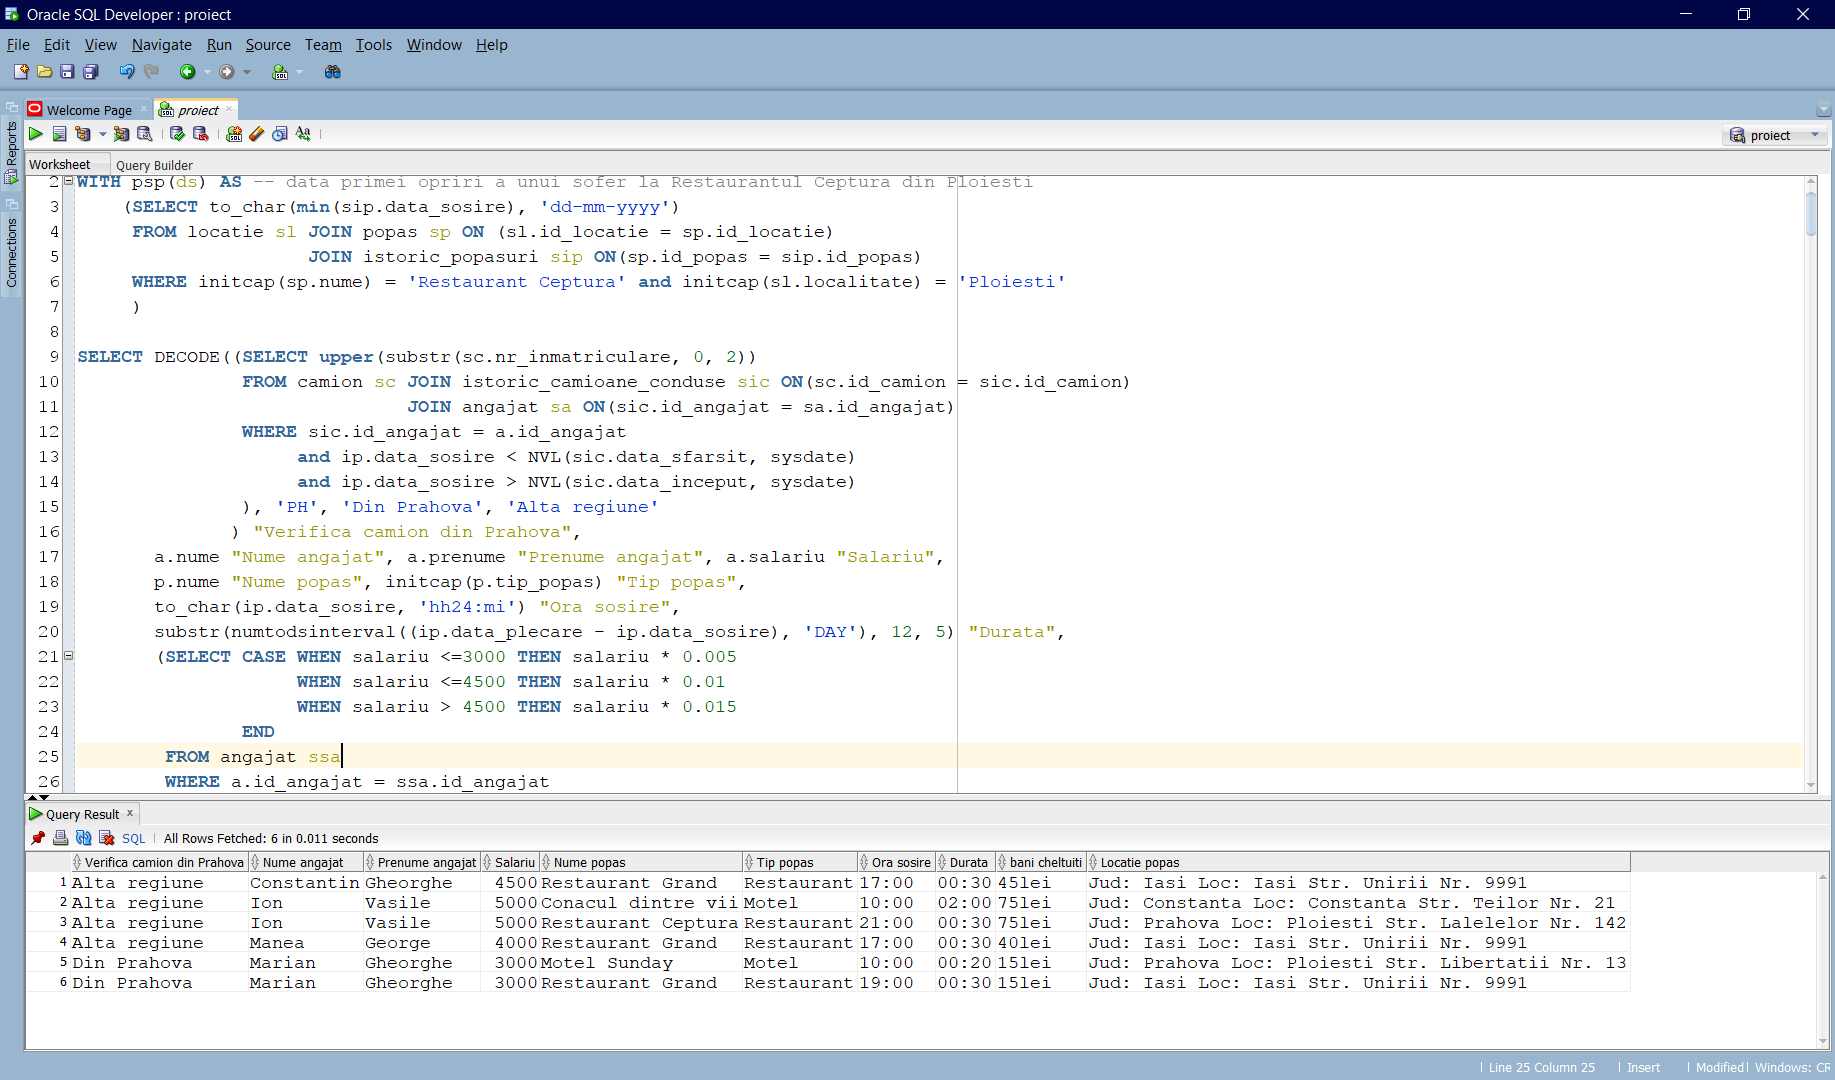
\includegraphics[width=\textwidth]{ex11_1.PNG}
\label{Ex11 1}
\centering Ex. 11 - 1

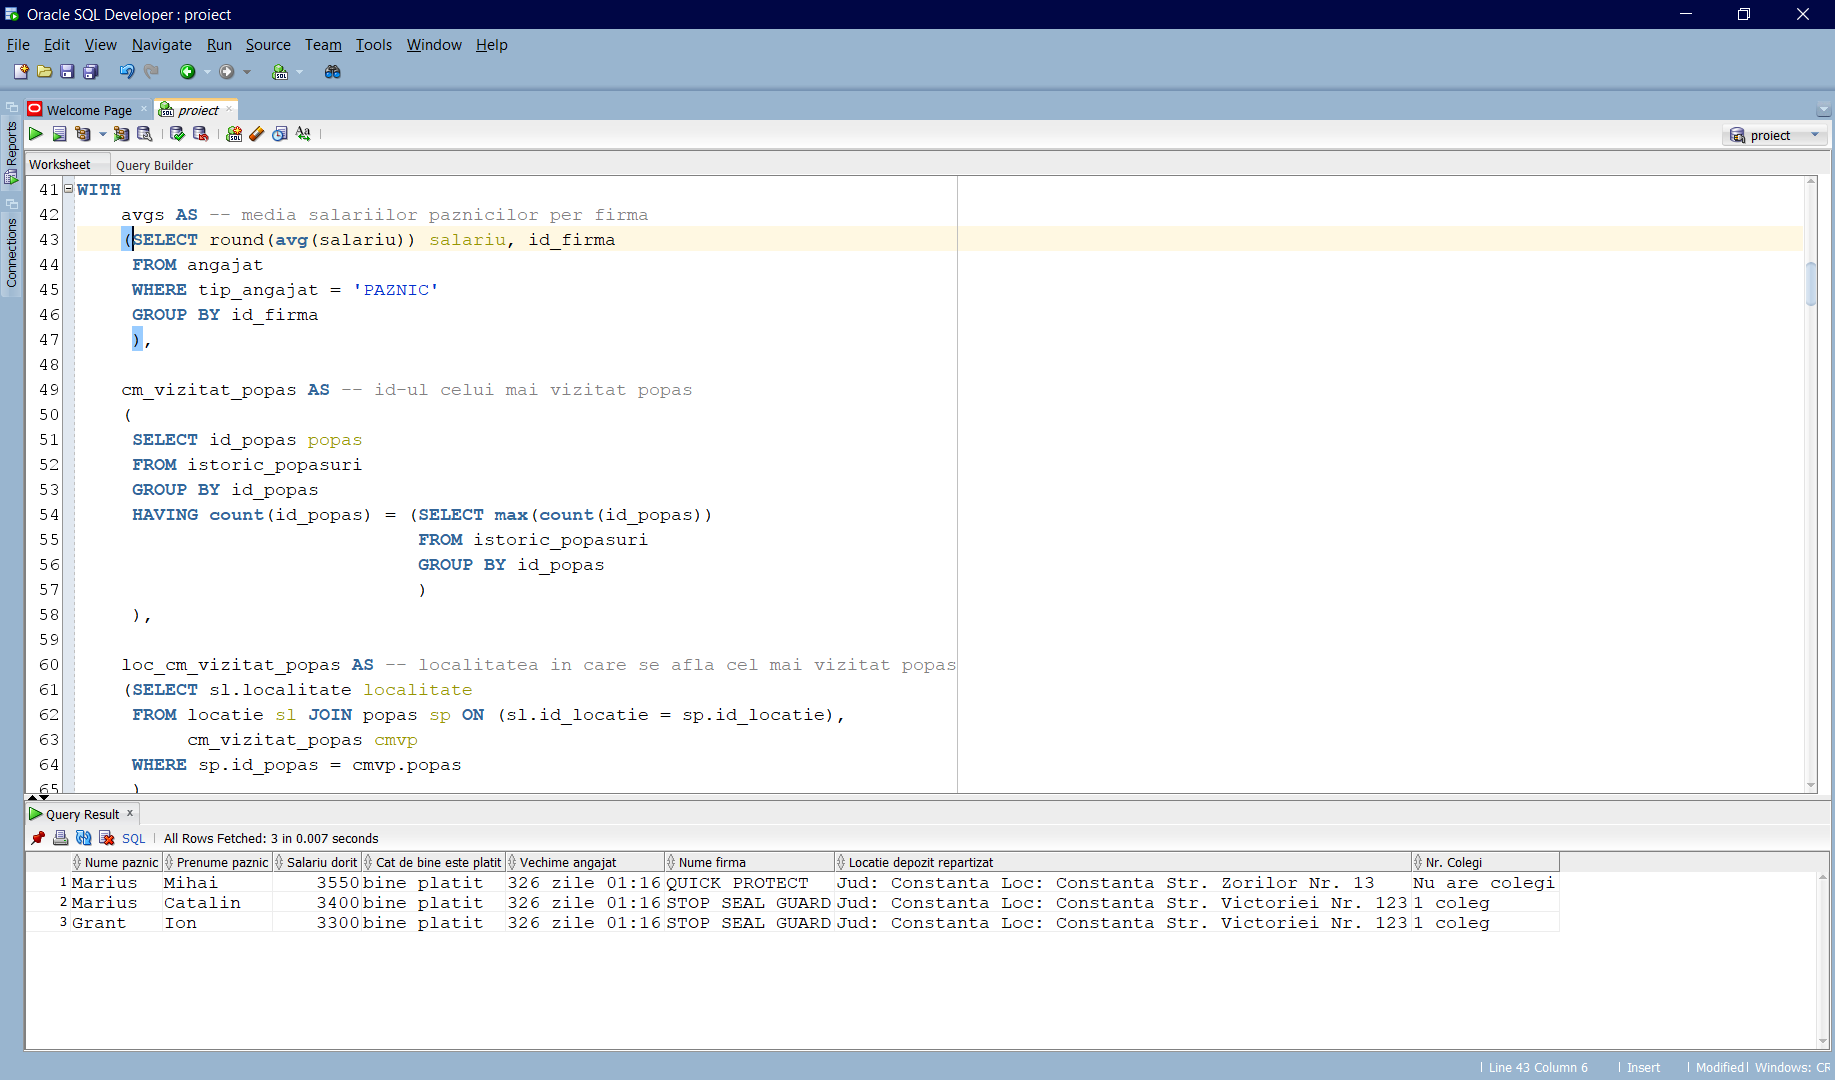
\includegraphics[width=\textwidth]{ex11_2.PNG}
\label{Ex11 2}
\centering Ex. 11 - 2

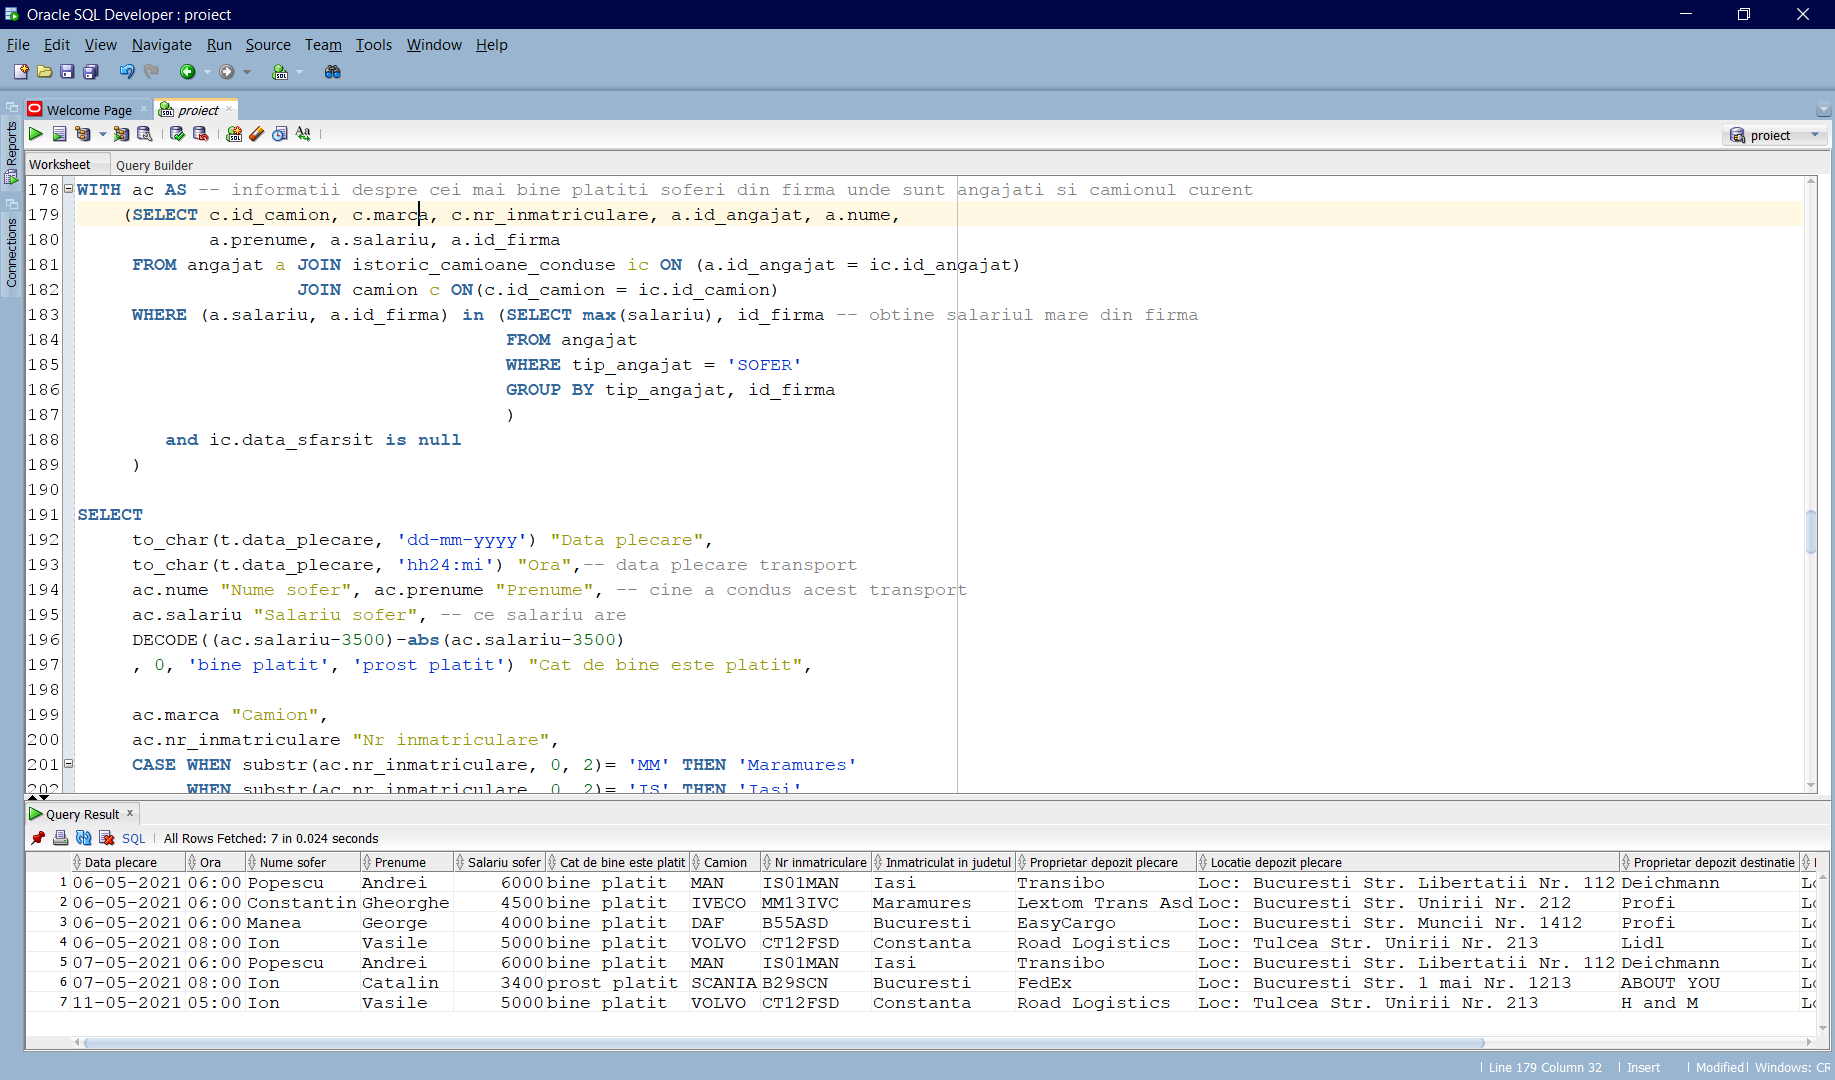
\includegraphics[width=\textwidth]{ex11_3_1.PNG}
\label{Ex11 3.1}
\centering Ex. 11 - 3.1

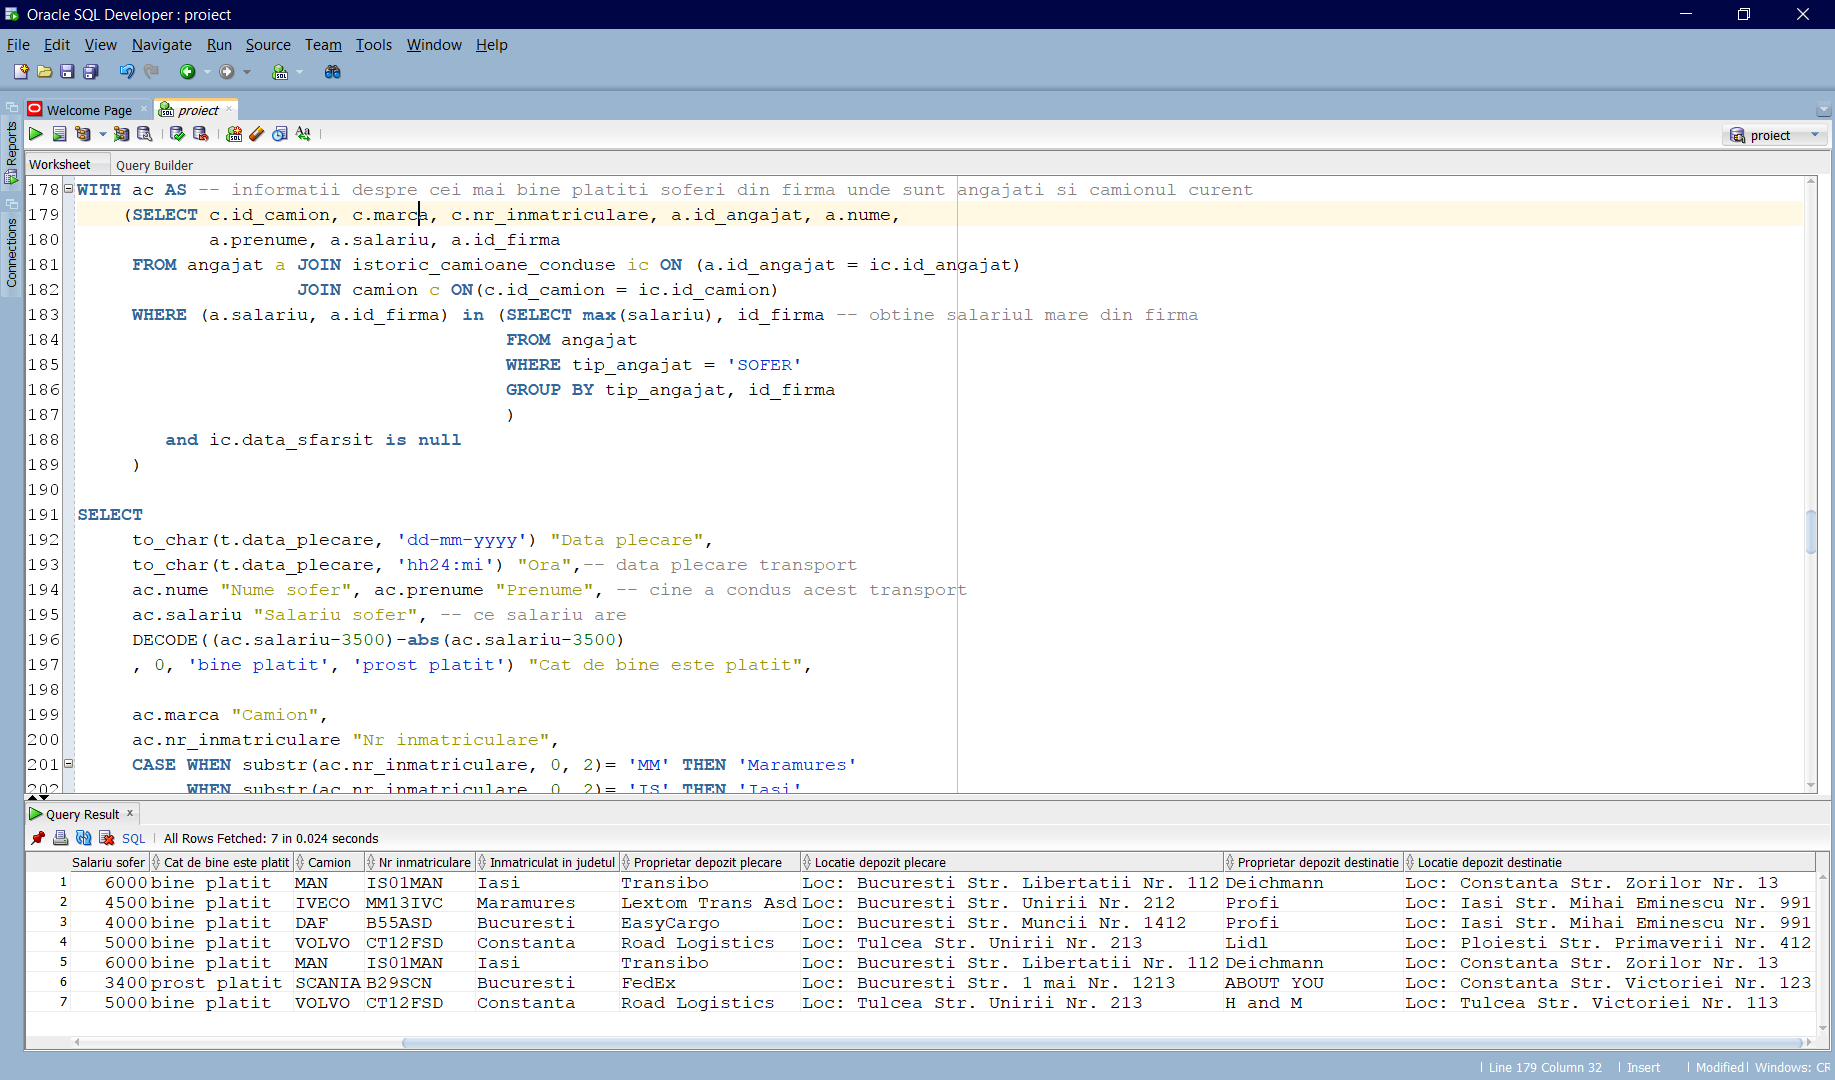
\includegraphics[width=\textwidth]{ex11_3_2.PNG}
\label{Ex11 3.2}
\centering Ex. 11 - 3.2

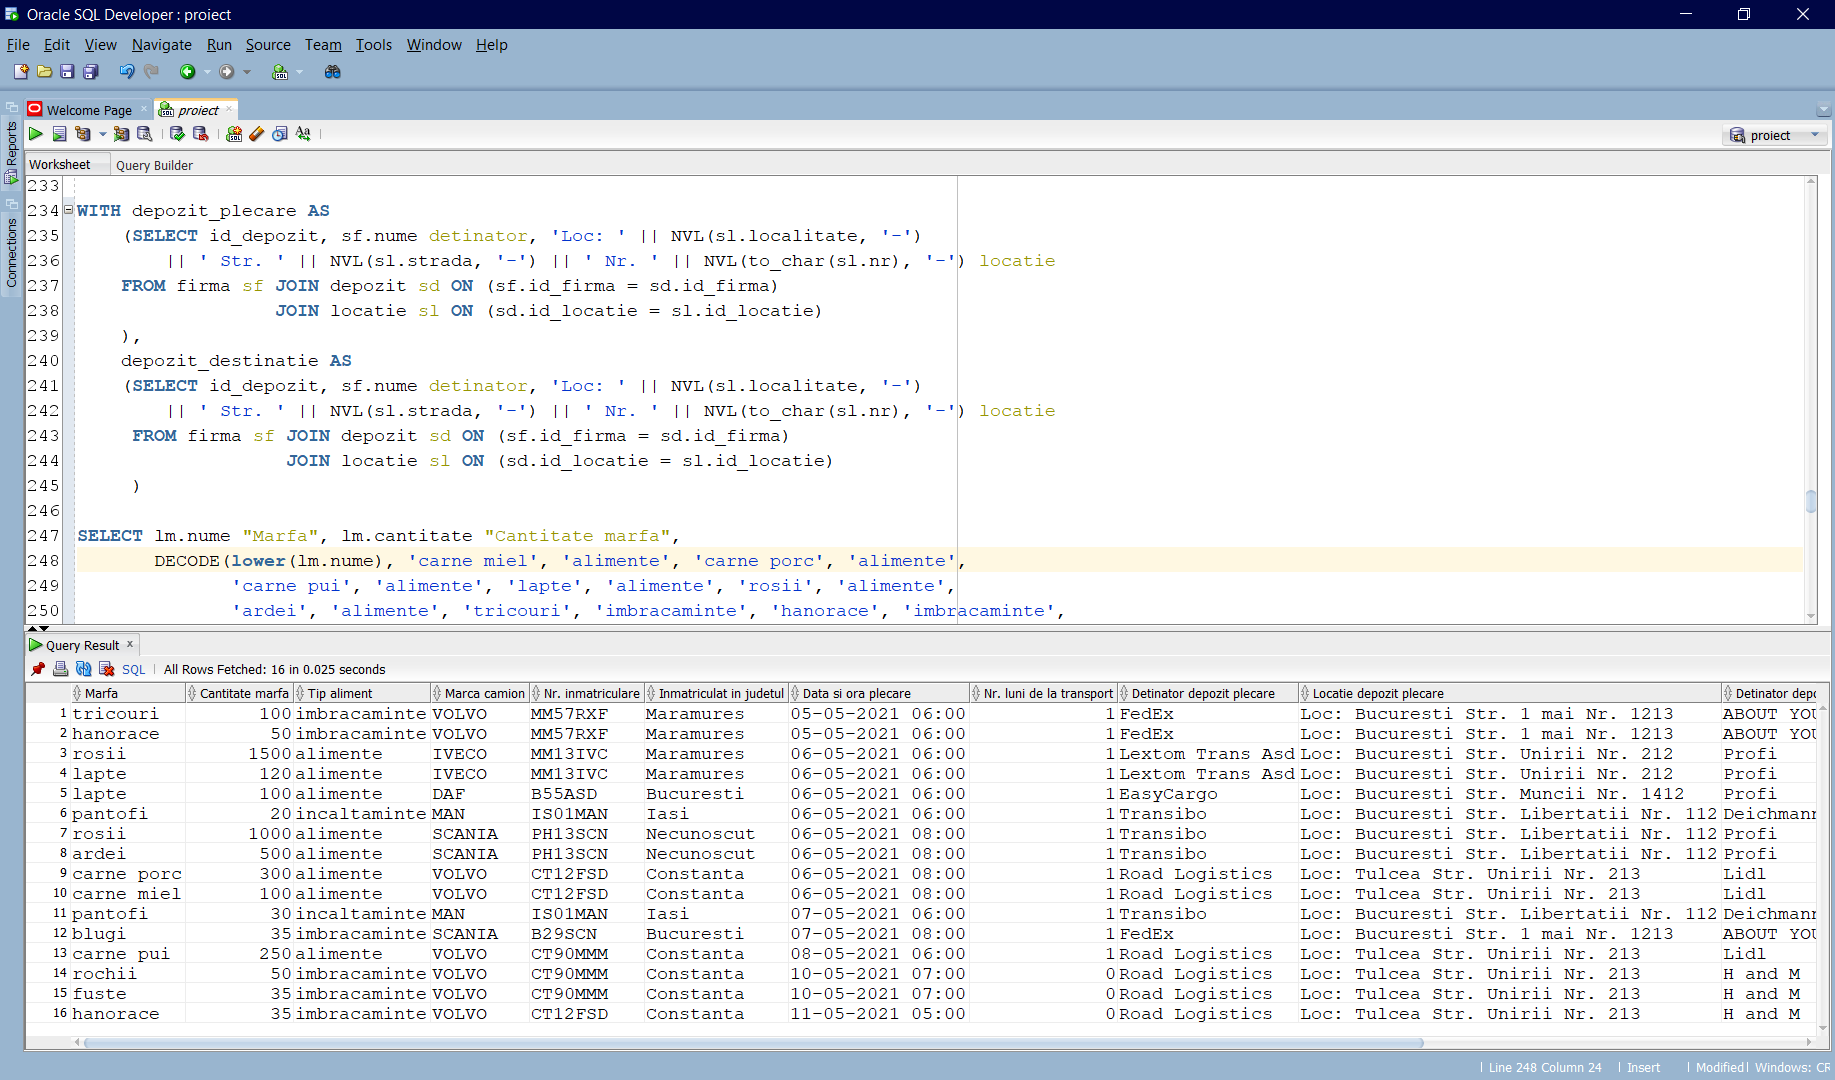
\includegraphics[width=\textwidth]{ex11_4_1.PNG}
\label{Ex11 4.1}
\centering Ex. 11 - 4.1

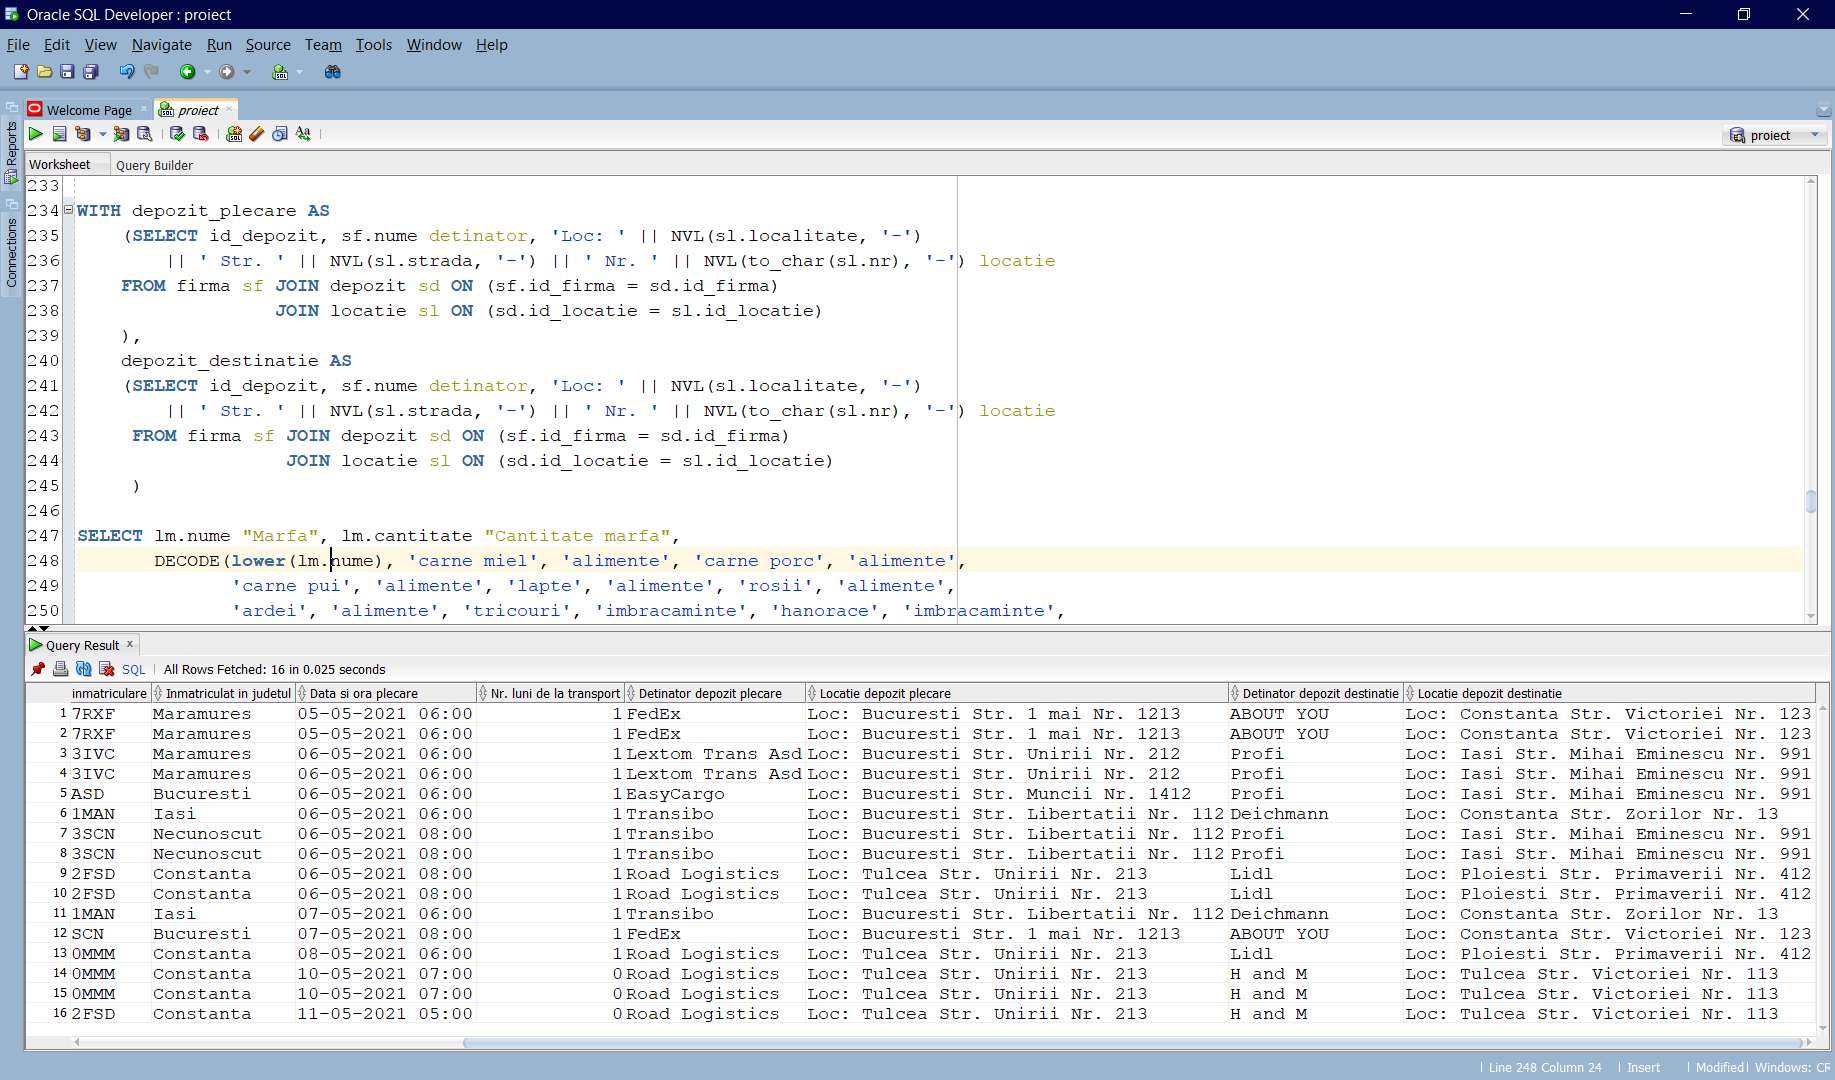
\includegraphics[width=\textwidth]{ex11_4_2.PNG}
\label{Ex11 4.2}
\centering Ex. 11 - 4.2

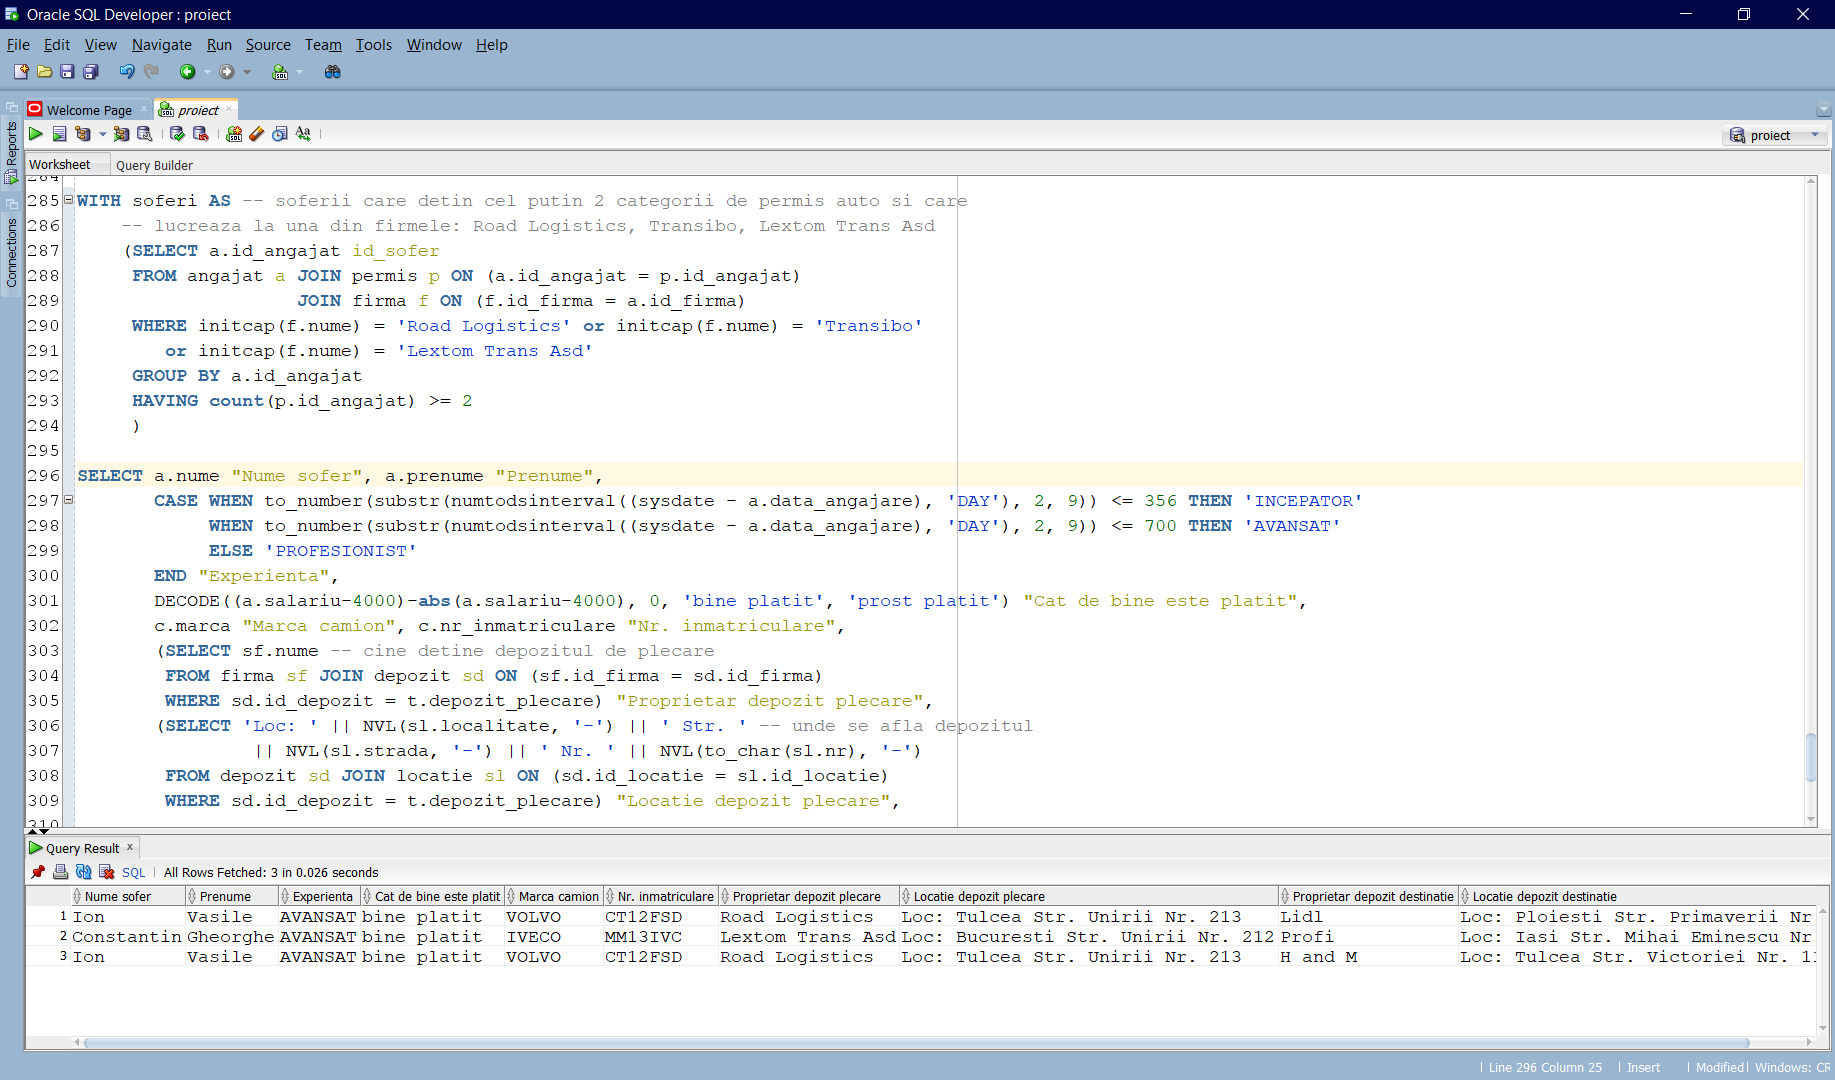
\includegraphics[width=\textwidth]{ex11_5.PNG}
\label{Ex11 5}
\centering Ex. 11 - 5

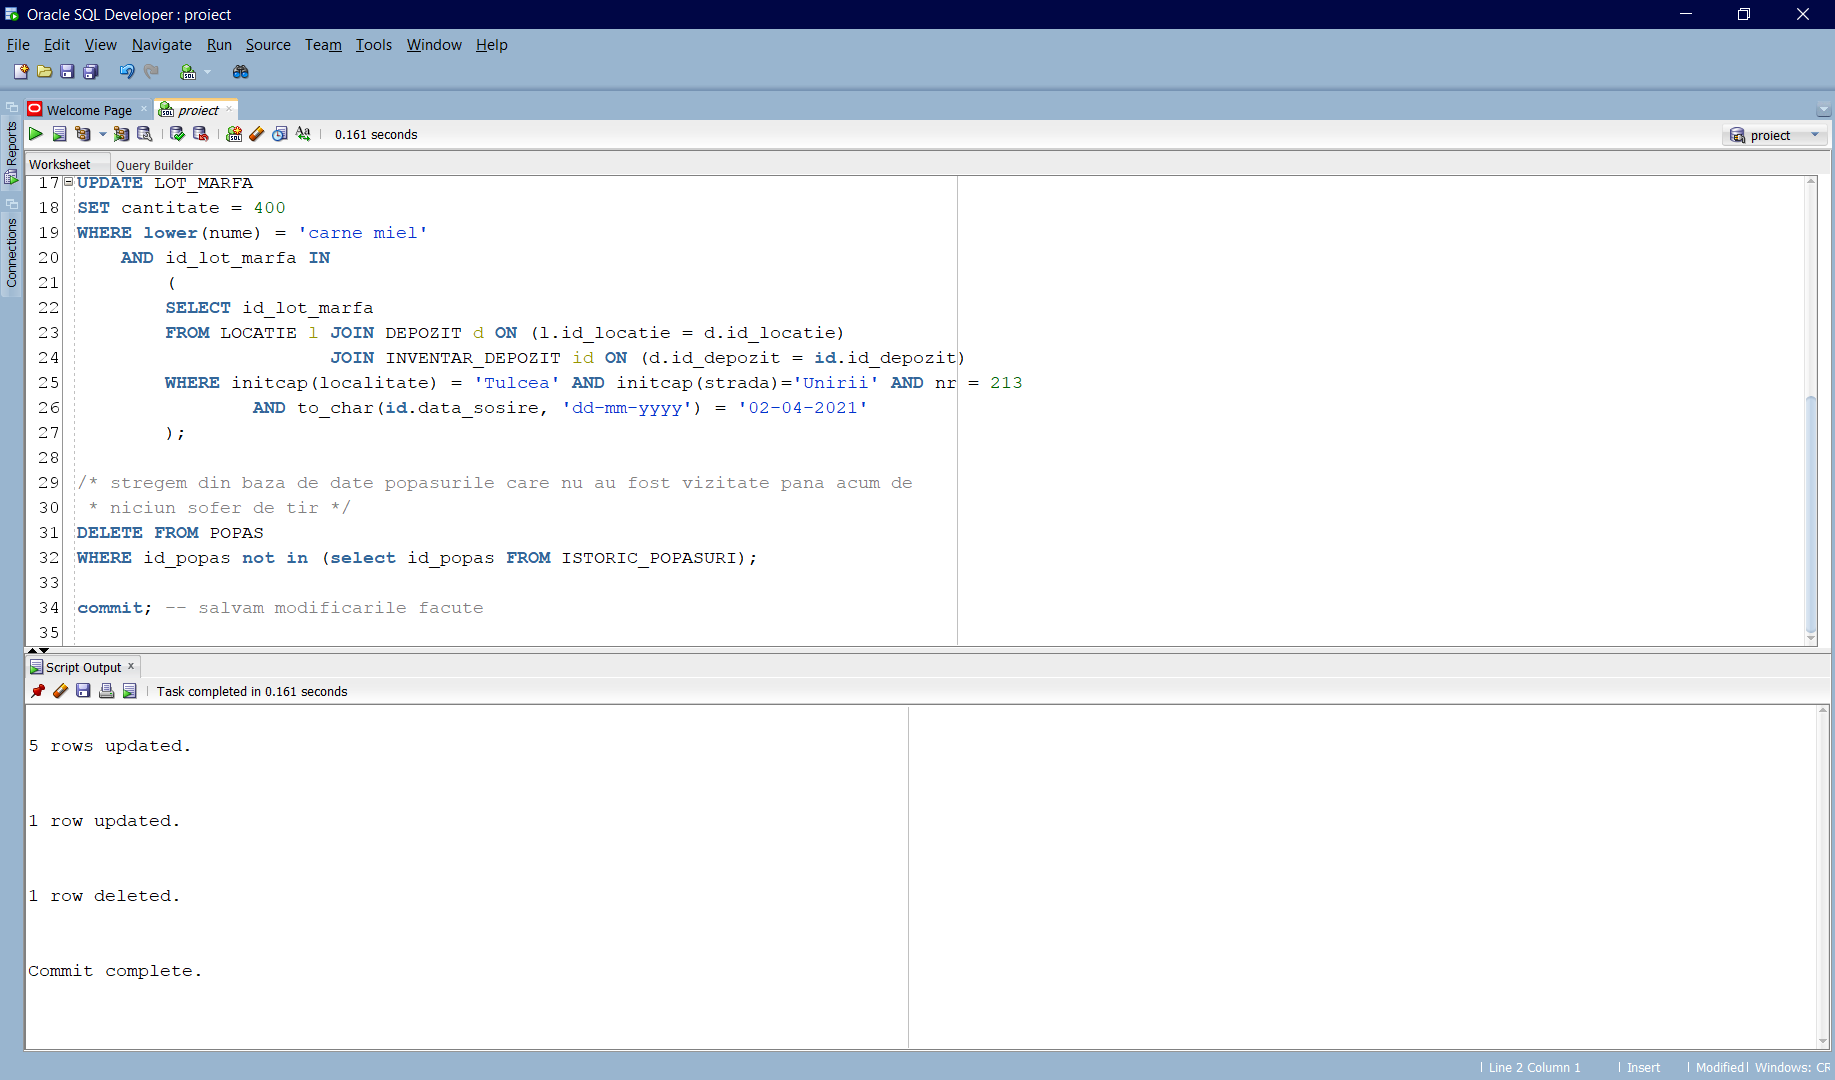
\includegraphics[width=\textwidth]{ex12.PNG}
\label{Ex12}
\centering Ex. 12 - 2 updateuri + 1 delete urmate de commit

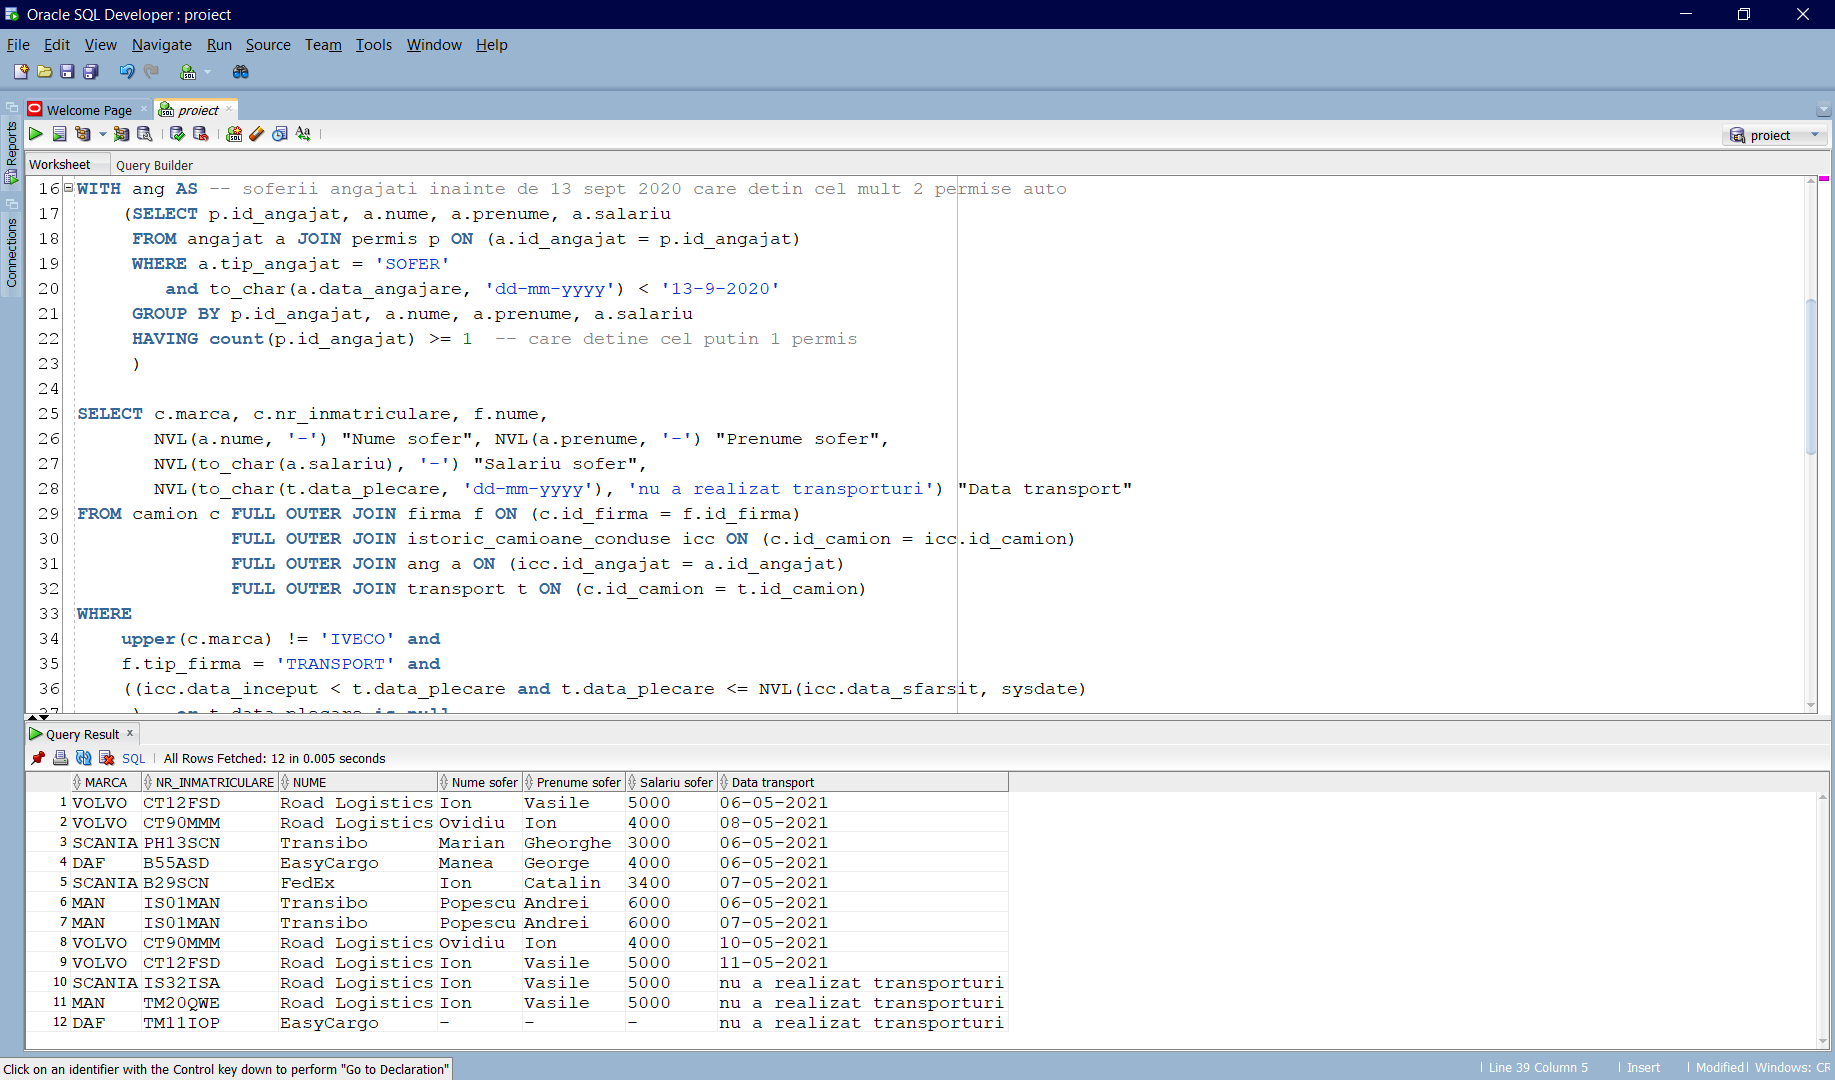
\includegraphics[width=\textwidth]{outer_join_1.PNG}
\label{Ex16 1-1}
\centering Ex. 16 - 1v1 outer join

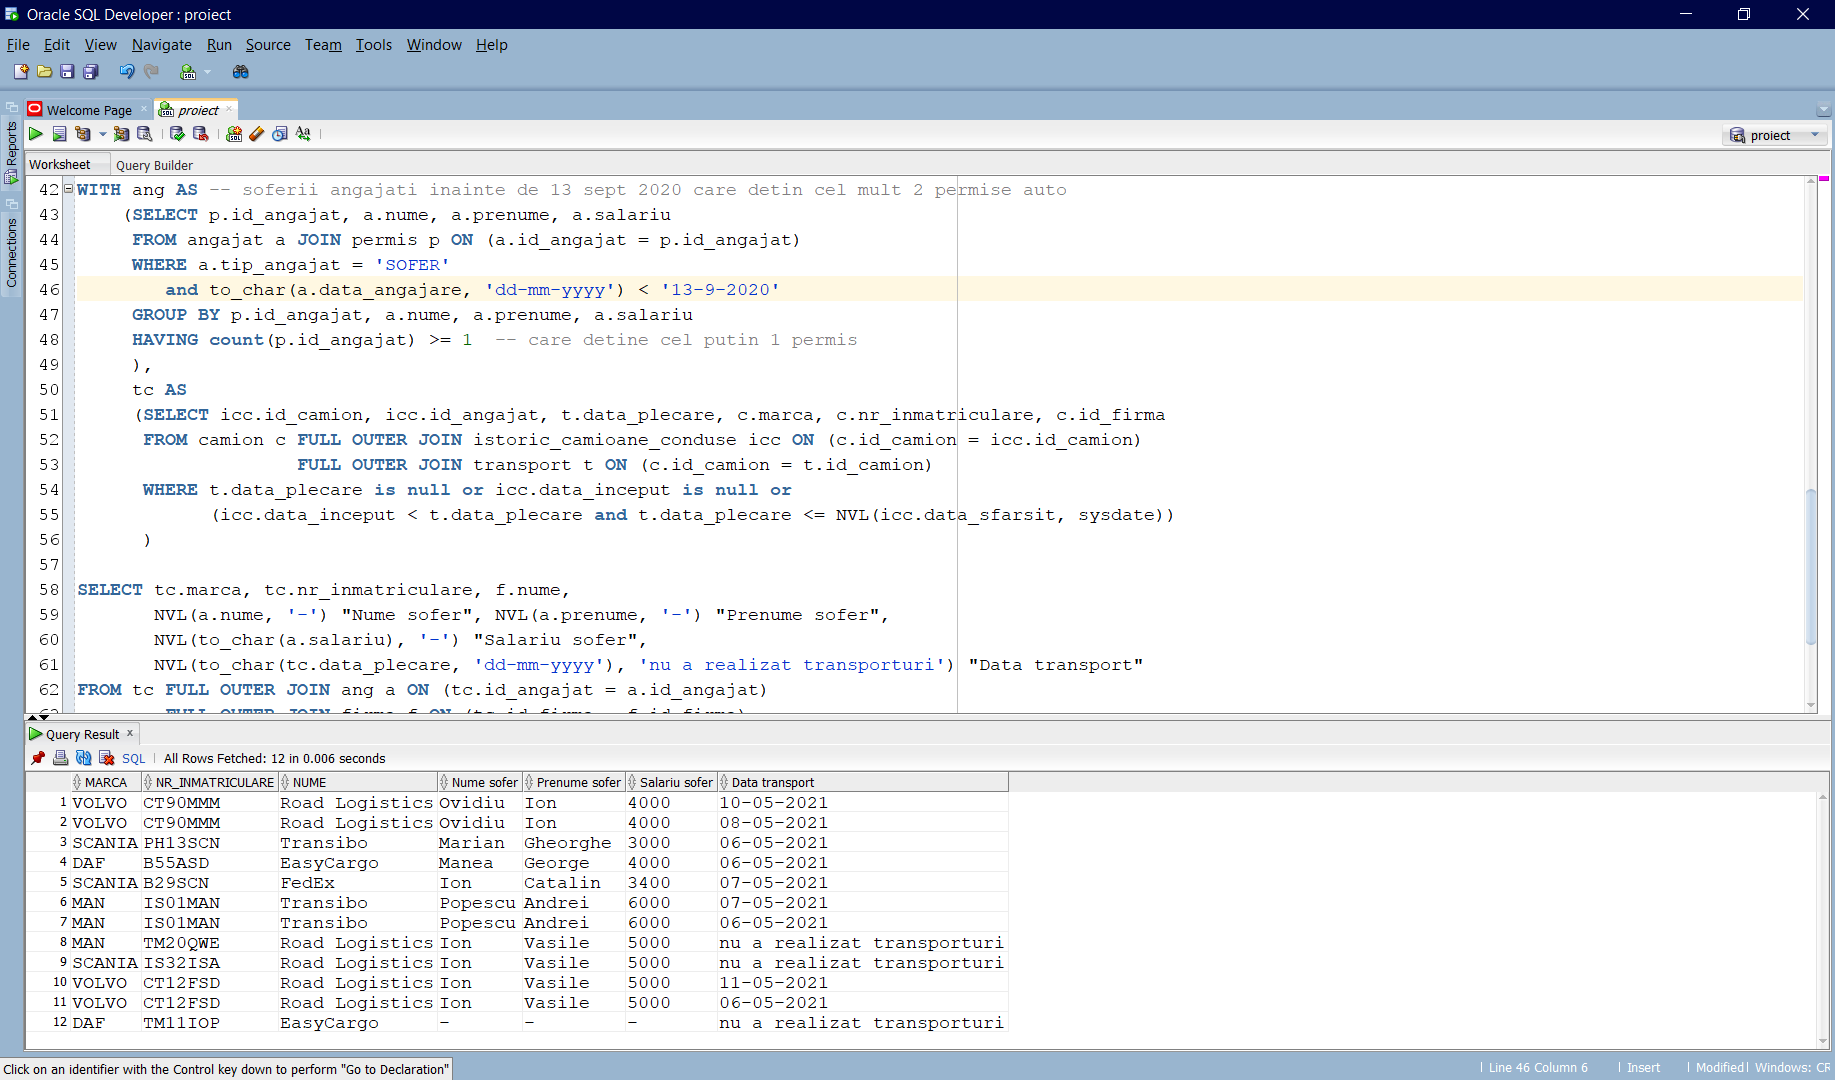
\includegraphics[width=\textwidth]{outer_join_2.PNG}
\label{Ex16 1-2}
\centering Ex. 16 - 1v2 outer join versiune îmbunătățită

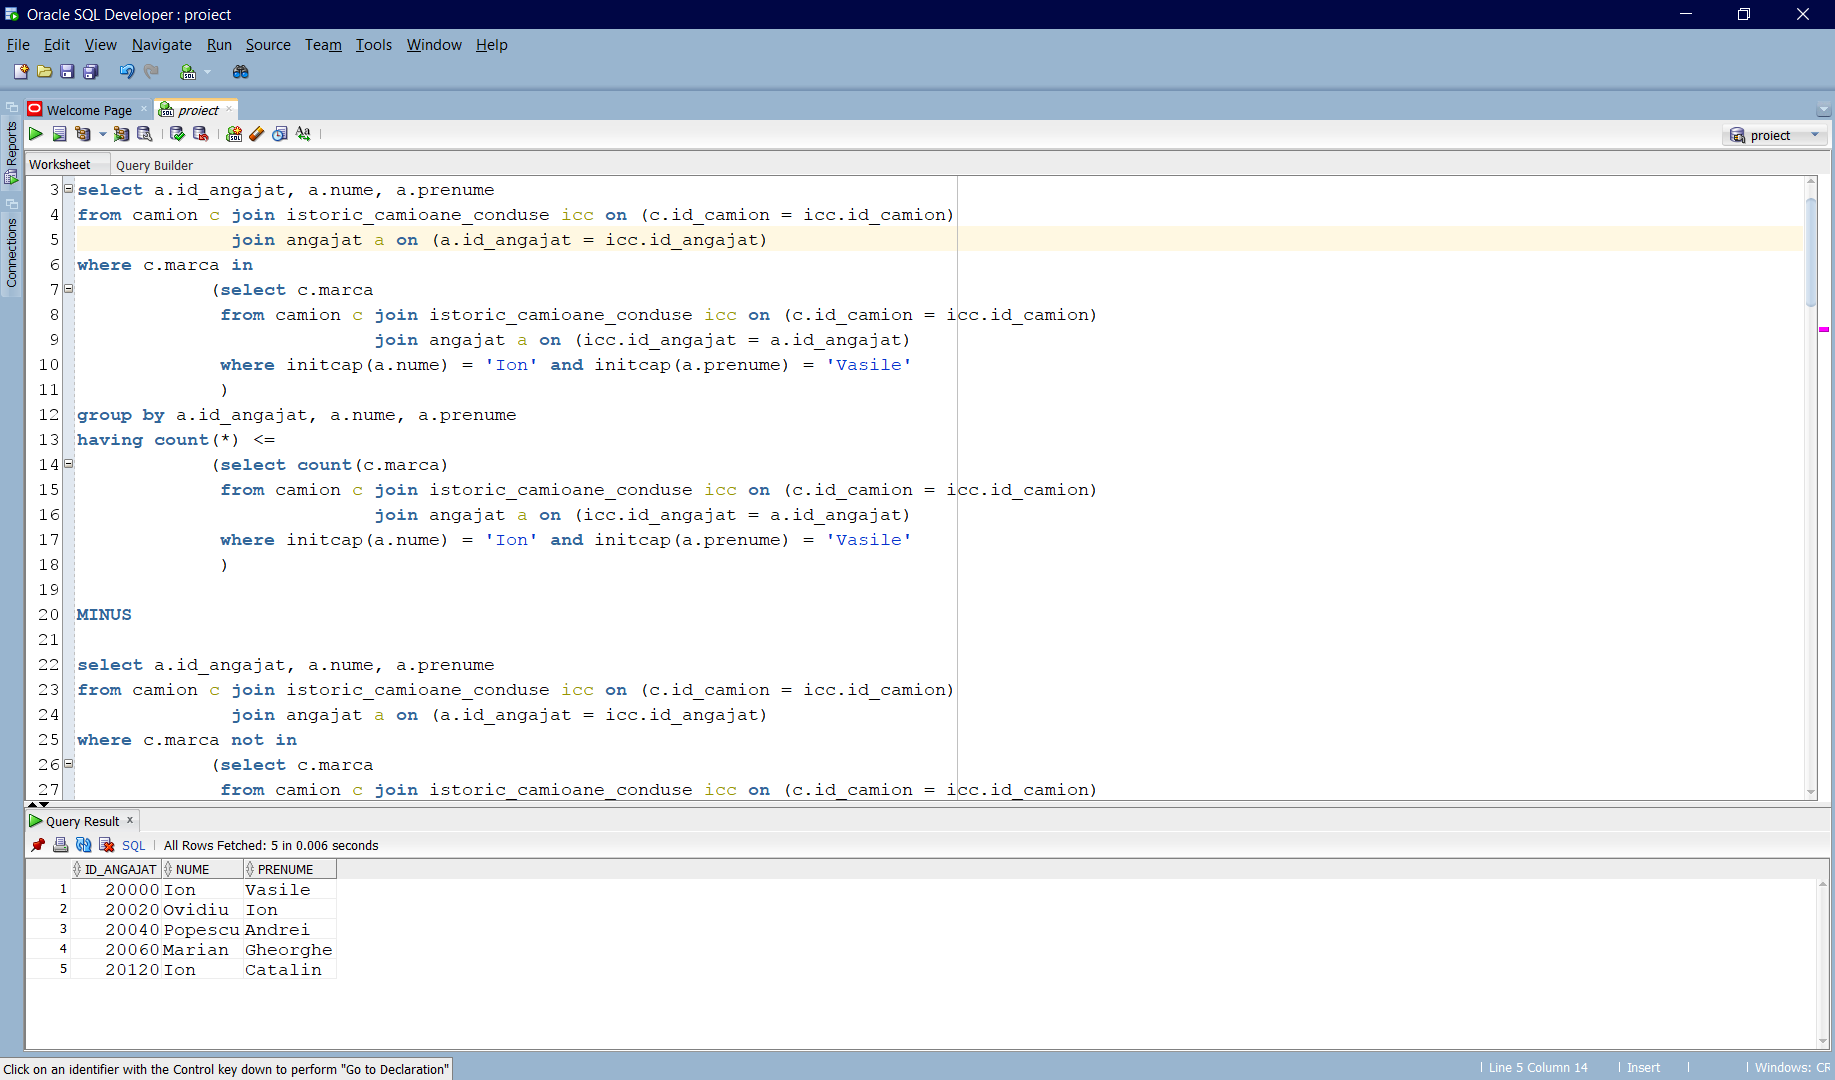
\includegraphics[width=\textwidth]{division_1.PNG}
\label{Ex16 2-1}
\centering Ex. 16 - 2-1 division

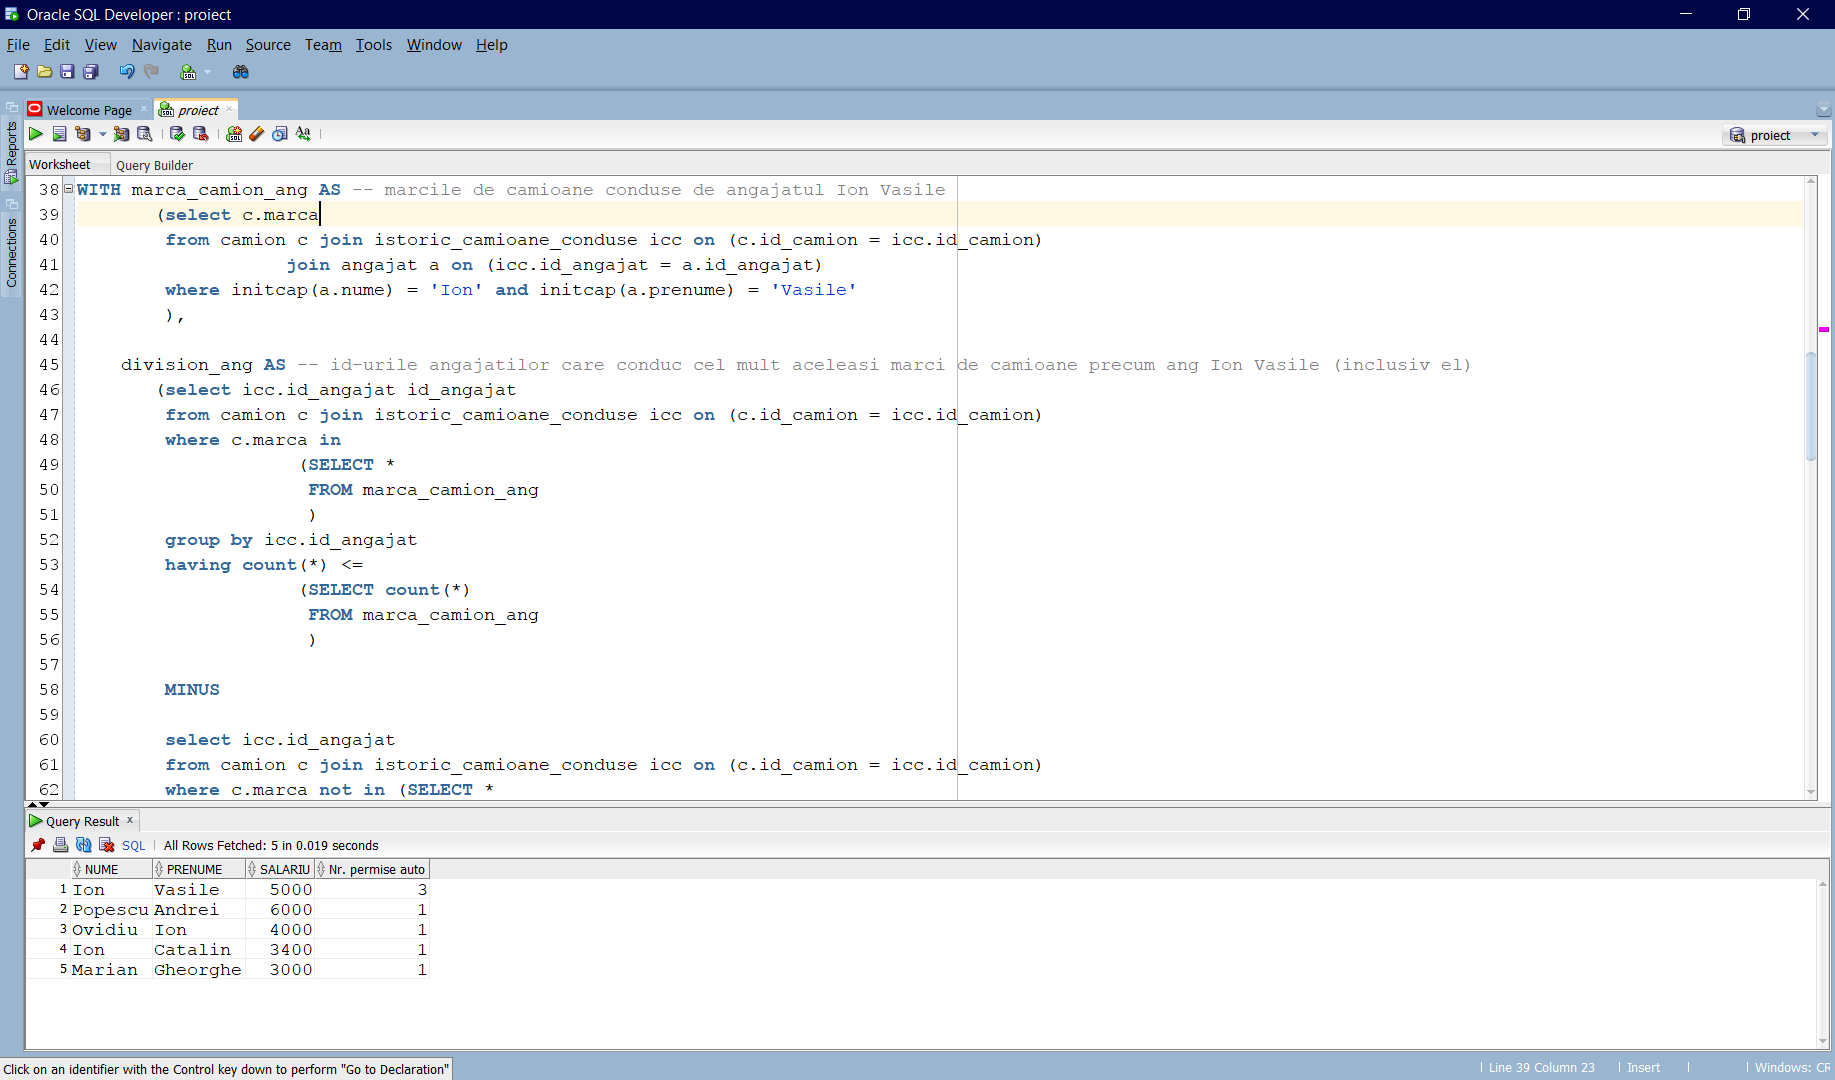
\includegraphics[width=\textwidth]{division_2.PNG}
\label{Ex16 2-2}
\centering Ex. 16 - 2-2 division

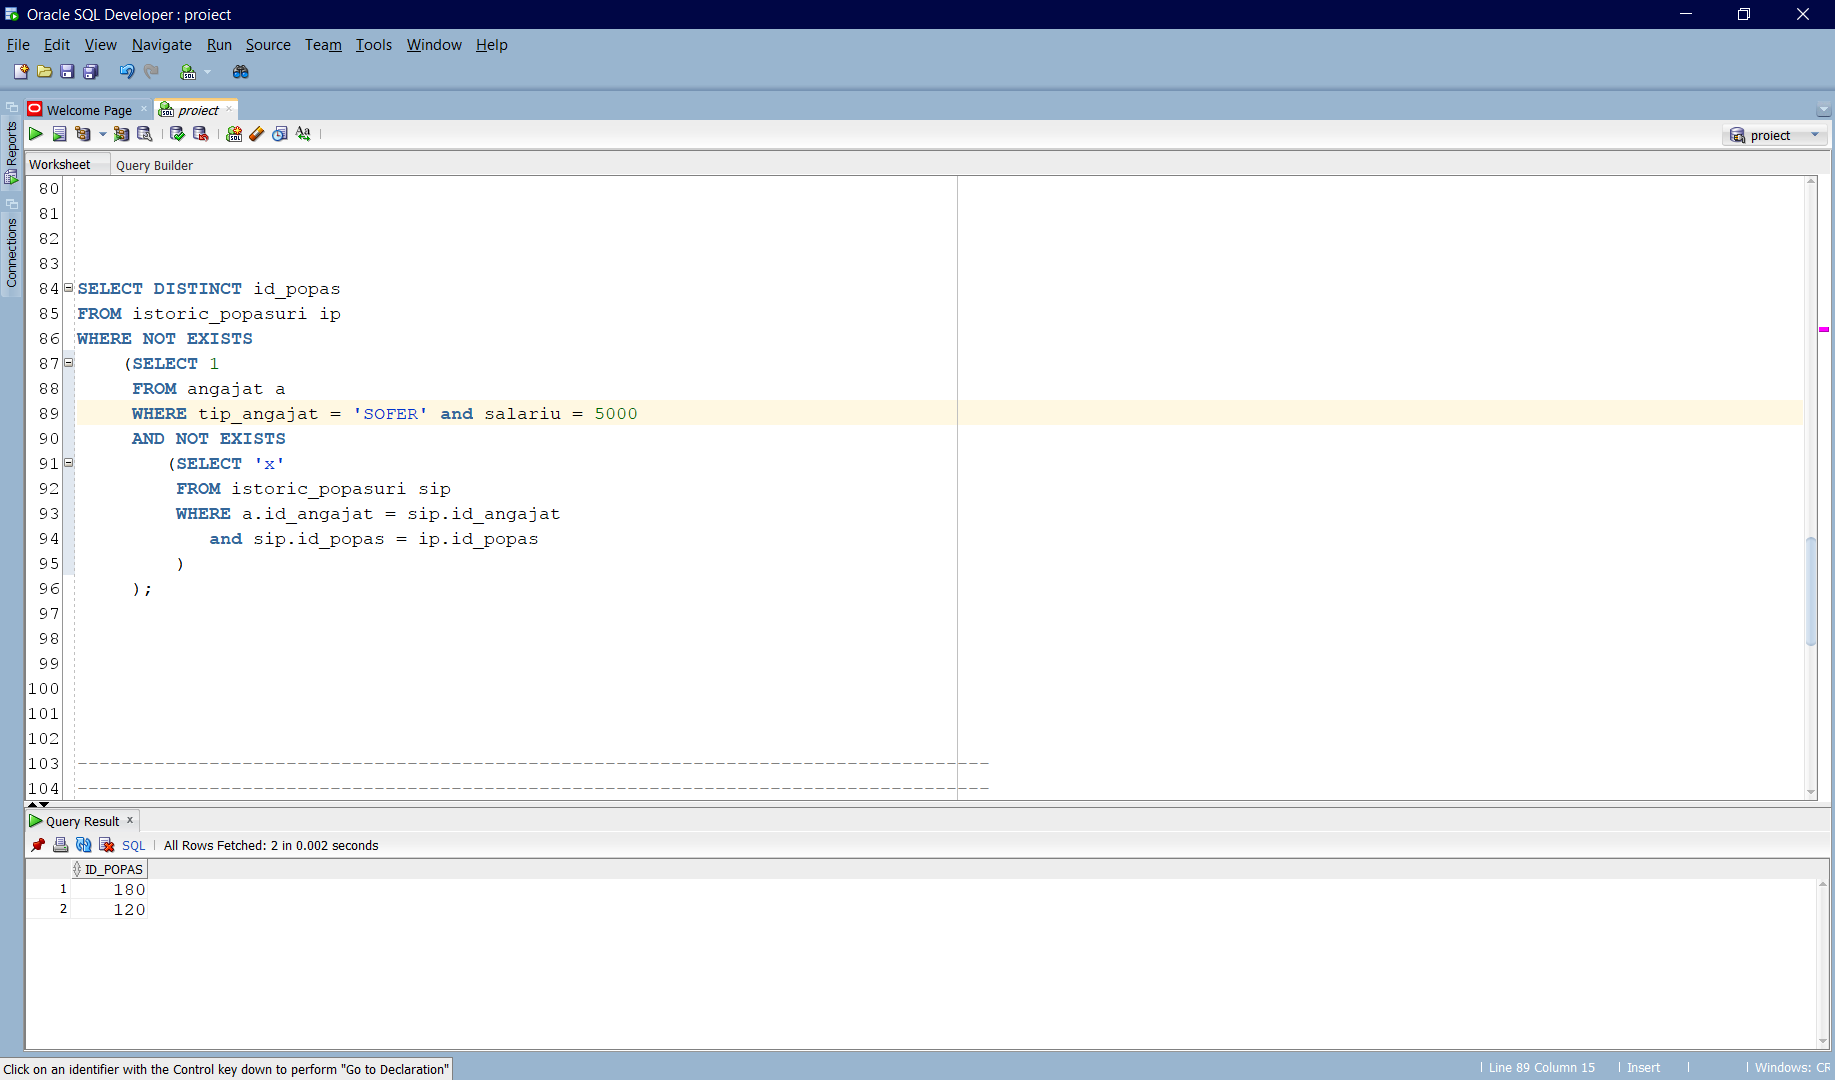
\includegraphics[width=\textwidth]{division_3.PNG}
\label{Ex16 2-3}
\centering Ex. 16 - 2-3 division

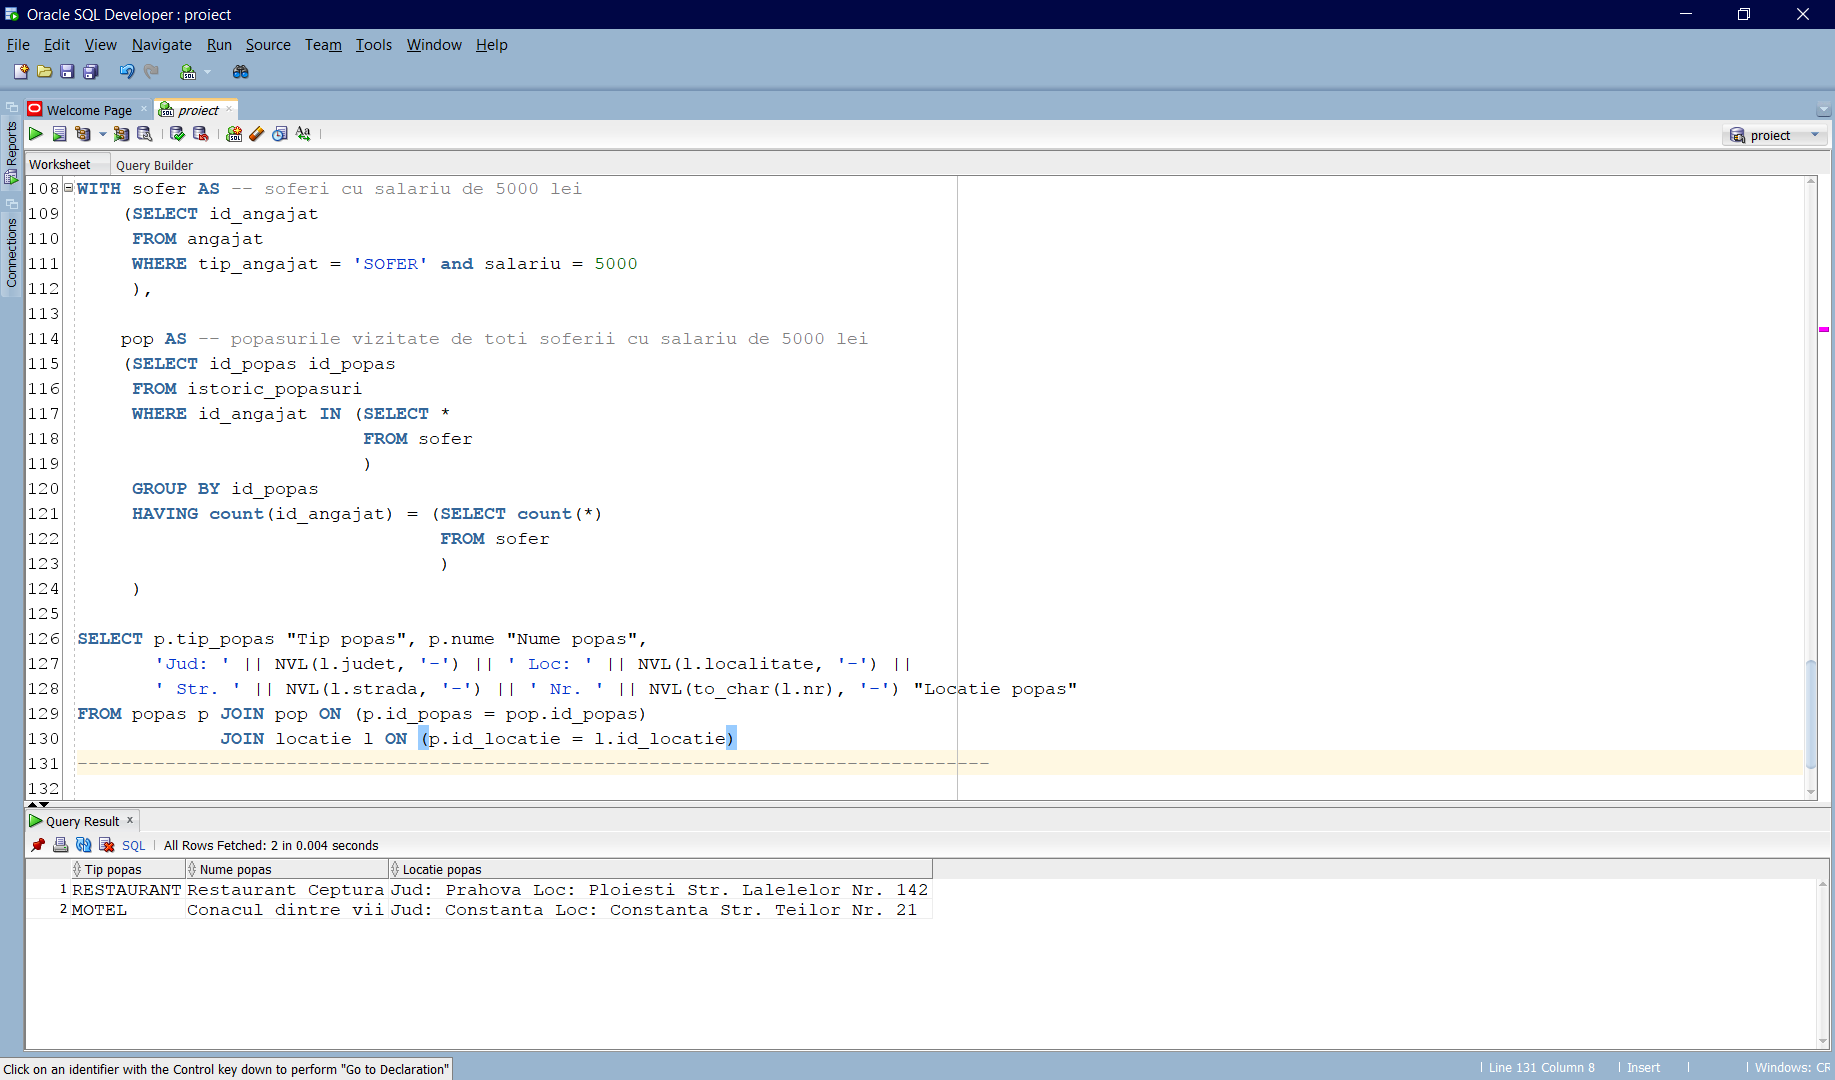
\includegraphics[width=\textwidth]{division_4.PNG}
\label{Ex16 2-4}
\centering Ex. 16 - 2-4 division


\end{document}
